%%%%%%%%%%%%%%%%%%%%%%%%%%%%%%%%%%%%%%%%%%%%%%%%%%%%%%%%%%%%%%%%%%
% Built from ITSS_Template/root.tex (IEEEtran conference class). Compile from this folder:
%   pdflatex main && bibtex main && pdflatex main && pdflatex main
% Sections live in sections/*.tex, figures in figures/, generated tables in tables/.
\documentclass[conference]{IEEEtran}
\IEEEoverridecommandlockouts

\usepackage{multirow}
\usepackage{amsmath}
\usepackage{amssymb}
\usepackage{graphicx}
\usepackage{booktabs}
\usepackage{array}
\usepackage{url}
\usepackage[hidelinks]{hyperref}
\graphicspath{{./figures/}}

\title{\LARGE \bf Reading Vehicle Size and Powertrain from Motion: A Trajectory--CAN Benchmark with Held-Out Car Models, Pre-Registered Methods and Label Ceilings}

% Anonymity switch: \anonymoustrue hides the author block and the repository links (double-blind submission);
% \anonymousfalse prints them (camera-ready). Author list given by the authors on 8 Nov 2026.
\newif\ifanonymous
% default: anonymous (target venue IEEE IV: double-blind review); build the author version with
%   pdflatex -jobname=main_authors "\def\withauthors{1}%%%%%%%%%%%%%%%%%%%%%%%%%%%%%%%%%%%%%%%%%%%%%%%%%%%%%%%%%%%%%%%%%%
% Built from ITSS_Template/root.tex (IEEEtran conference class). Compile from this folder:
%   pdflatex main && bibtex main && pdflatex main && pdflatex main
% Sections live in sections/*.tex, figures in figures/, generated tables in tables/.
\documentclass[conference]{IEEEtran}
\IEEEoverridecommandlockouts

\usepackage{multirow}
\usepackage{amsmath}
\usepackage{amssymb}
\usepackage{graphicx}
\usepackage{booktabs}
\usepackage{array}
\usepackage{url}
\usepackage[hidelinks]{hyperref}
\graphicspath{{./figures/}}

\title{\LARGE \bf Reading Vehicle Size and Powertrain from Motion: A Trajectory--CAN Benchmark with Held-Out Car Models, Pre-Registered Methods and Label Ceilings}

% Anonymity switch: \anonymoustrue hides the author block and the repository links (double-blind submission);
% \anonymousfalse prints them (camera-ready). Author list given by the authors on 8 Nov 2026.
\newif\ifanonymous
% default: anonymous (target venue IEEE IV: double-blind review); build the author version with
%   pdflatex -jobname=main_authors "\def\withauthors{1}%%%%%%%%%%%%%%%%%%%%%%%%%%%%%%%%%%%%%%%%%%%%%%%%%%%%%%%%%%%%%%%%%%
% Built from ITSS_Template/root.tex (IEEEtran conference class). Compile from this folder:
%   pdflatex main && bibtex main && pdflatex main && pdflatex main
% Sections live in sections/*.tex, figures in figures/, generated tables in tables/.
\documentclass[conference]{IEEEtran}
\IEEEoverridecommandlockouts

\usepackage{multirow}
\usepackage{amsmath}
\usepackage{amssymb}
\usepackage{graphicx}
\usepackage{booktabs}
\usepackage{array}
\usepackage{url}
\usepackage[hidelinks]{hyperref}
\graphicspath{{./figures/}}

\title{\LARGE \bf Reading Vehicle Size and Powertrain from Motion: A Trajectory--CAN Benchmark with Held-Out Car Models, Pre-Registered Methods and Label Ceilings}

% Anonymity switch: \anonymoustrue hides the author block and the repository links (double-blind submission);
% \anonymousfalse prints them (camera-ready). Author list given by the authors on 8 Nov 2026.
\newif\ifanonymous
% default: anonymous (target venue IEEE IV: double-blind review); build the author version with
%   pdflatex -jobname=main_authors "\def\withauthors{1}%%%%%%%%%%%%%%%%%%%%%%%%%%%%%%%%%%%%%%%%%%%%%%%%%%%%%%%%%%%%%%%%%%
% Built from ITSS_Template/root.tex (IEEEtran conference class). Compile from this folder:
%   pdflatex main && bibtex main && pdflatex main && pdflatex main
% Sections live in sections/*.tex, figures in figures/, generated tables in tables/.
\documentclass[conference]{IEEEtran}
\IEEEoverridecommandlockouts

\usepackage{multirow}
\usepackage{amsmath}
\usepackage{amssymb}
\usepackage{graphicx}
\usepackage{booktabs}
\usepackage{array}
\usepackage{url}
\usepackage[hidelinks]{hyperref}
\graphicspath{{./figures/}}

\title{\LARGE \bf Reading Vehicle Size and Powertrain from Motion: A Trajectory--CAN Benchmark with Held-Out Car Models, Pre-Registered Methods and Label Ceilings}

% Anonymity switch: \anonymoustrue hides the author block and the repository links (double-blind submission);
% \anonymousfalse prints them (camera-ready). Author list given by the authors on 8 Nov 2026.
\newif\ifanonymous
% default: anonymous (target venue IEEE IV: double-blind review); build the author version with
%   pdflatex -jobname=main_authors "\def\withauthors{1}\input{main}"
\ifdefined\withauthors\anonymousfalse\else\anonymoustrue\fi

\ifanonymous
\author{\parbox{\textwidth}{\centering Author names withheld for review}}
\else
\author{%
	\parbox{\textwidth}{%
		\centering
		Yuhang Wang, Yuechen Guo, Jingxin Yang, Chuheng Wei, Suyang Chen,\\
		Abdulaziz Alhuraish, Yiyi Wang, Jingran Sun and Hao Zhou%
	}%
	% TODO (authors): affiliations and contact e-mails, e.g.
	% \thanks{$^{1}$Affiliation 1, City, Country {\tt\small contact address}}
}
\fi

\begin{document}
\maketitle
\thispagestyle{empty}
\pagestyle{empty}

\input{sections/00_abstract}
\input{sections/01_intro}
\input{sections/02_related}
\input{sections/03_dataset}
\input{sections/04_methods}
\input{sections/05_experiments}
\input{sections/06_discussion}
\input{sections/07_conclusion}

\ifanonymous\else
\section*{Acknowledgments}
% TODO (authors): funding and acknowledgments, or remove.
\fi

\bibliographystyle{IEEEtran}
\bibliography{refs}

\end{document}
"
\ifdefined\withauthors\anonymousfalse\else\anonymoustrue\fi

\ifanonymous
\author{\parbox{\textwidth}{\centering Author names withheld for review}}
\else
\author{%
	\parbox{\textwidth}{%
		\centering
		Yuhang Wang, Yuechen Guo, Jingxin Yang, Chuheng Wei, Suyang Chen,\\
		Abdulaziz Alhuraish, Yiyi Wang, Jingran Sun and Hao Zhou%
	}%
	% TODO (authors): affiliations and contact e-mails, e.g.
	% \thanks{$^{1}$Affiliation 1, City, Country {\tt\small contact address}}
}
\fi

\begin{document}
\maketitle
\thispagestyle{empty}
\pagestyle{empty}

\begin{abstract}
Trajectory data for traffic analytics, simulation calibration and infrastructure studies rarely record the vehicle type. We ask whether it can be read from motion alone: can 60-s windows of trajectory and CAN signals reveal the size class (three footprint classes) and the powertrain (battery-electric vs combustion, BEV vs ICE) of car models never seen in training? We release a pseudonymous dataset of 9,062 drives (about 3,950 h) from 1,431 vehicles and 174 car models, with held-out-car-model and held-out-device splits, window-, drive- and vehicle-level protocols and cluster-bootstrap intervals over car models. Four sequence architectures (ResNet, bi-GRU, Transformer, Mamba-2), hand-crafted statistics and physical features proposed by large language models (LLMs) serve as reference points; a pre-registered method study on model-disjoint internal folds adds car-model-balanced sampling, auxiliary physical targets, physics-safe augmentation, per-car-model loss re-weighting and, for BEV vs ICE, down-weighting of driving automation system (DAS) periods. On held-out car models, BEV vs ICE reaches 92.6--93.0 drive-level macro-F1 (95\% interval [87.1, 96.2] for the final bi-GRU); size improves from 62.9 to 67.1 at drive level but stays far from 90. Run unchanged on a public fleet of 4,061 devices absent from our library, the final models call the powertrain right for 86 of 88 car models and match the internal size result (63.2\% of devices against 63.5\% at vehicle level). Zero-training oracle analyses attribute the gap to label resolution and training-fleet composition rather than to evidence per drive; the architecture benchmark shows model capacity is not the bottleneck.
\end{abstract}
% W1: shorter title alternative, if wanted:
% "Reading Vehicle Size and Powertrain from Motion: A Trajectory--CAN Benchmark with Held-Out Car Models"

\section{Introduction}\label{sec:intro}

Vehicle trajectories are collected at scale by roadside sensors, connected-vehicle platforms and aftermarket loggers, usually without a reliable record of the vehicle that produced them. Many uses need it: traffic analytics by vehicle class, calibration of microscopic simulation models whose car-following parameters differ between a compact car and a three-row SUV, and infrastructure studies of how often heavy or electric vehicles use a facility. Registration records, licence plates or camera images can fill the gap but raise privacy and availability problems; a trajectory that reveals its vehicle type by itself would be more privacy-friendly.

Motion should carry this information: wheelbase, steering ratio and mass distribution set the yaw and curvature response to steering, and the powertrain shapes launches and lift-off deceleration, so a battery-electric vehicle (BEV) braking largely through its motor should leave a different speed trace from an internal-combustion-engine (ICE) vehicle. We pose the question as it arises in deployment, for car models never seen in training, since otherwise every new model would need retraining. From 60-s windows of trajectory and controller area network (CAN) signals (among them speed, acceleration, steering, yaw rate, curvature, lateral acceleration, pedal and automation flags, and lead-vehicle distance, relative speed, headway and time-to-collision; Section~\ref{sec:dataset} lists all channels) we predict a size class (SMALL, MID or LARGE, cut from the vehicle footprint) and the powertrain (BEV vs ICE).

Three things make this hard. First, the size label is a hard cut through a continuous quantity (footprints of 4.43 and 4.88 m$^2$ separate the classes), so a car model near a cut is hard to place even when its physics is read well. Second, a driving automation system (DAS) is engaged in 47.9\%
of the samples, so part of the measured behaviour is a controller signature that may not transfer between car models. Third, the fleet is uneven (174 car models from 38 brands with widely differing hours), so a held-out model in a footprint gap of the training fleet has no neighbour to be read against.

We therefore release the data with fixed labels and splits, benchmark sequence models and feature pipelines under one protocol, run a pre-registered method study on model-disjoint folds, and ask, without training anything, where the size ceiling lies and why. The contributions are:

\begin{itemize}
\item A public, privacy-preserving trajectory and CAN dataset (9,062 drives, about 3,950 h, 1,431 pseudonymous vehicles) with fixed footprint-size and powertrain labels, held-out-car-model (headline) and held-out-device splits, and window-, drive- and vehicle-level protocols with cluster-bootstrap intervals over car models (Section~\ref{sec:dataset}).
\item A benchmark of four sequence architectures, hand-crafted statistics and physical features proposed by a large language model (LLM) under those protocols, showing that architecture is not the bottleneck (all deep models within about 2 points) and drive-level aggregation adds 7--12 points (Table~\ref{tab:main}).
\item A pre-registered method study on model-disjoint internal folds (Sections~\ref{sec:methods} and \ref{sec:experiments}): car-model-balanced sampling, auxiliary physical targets, physics-safe augmentation, per-car-model loss re-weighting (size) and DAS down-weighting (BEV vs ICE) raise the drive-level result by 4--6 points (size) and 2--4 points (BEV vs ICE); an episode-centric multiple-instance model over driving transients matches but does not beat the window recipes on the test models.
\item Zero-training ceiling analyses (per-car-model majority, footprint-noise and curb-mass oracles, evidence sufficiency, separability of held-out models) that quantify why size cannot reach 90 on unseen car models under a footprint cut, and what would make it reachable (Figs.~\ref{fig:evidence} and \ref{fig:ceiling}).
\end{itemize}

\section{Related Work}\label{sec:related}

\textbf{Electric and combustion vehicles on the road.} Battery-electric vehicles accelerate and slow down differently from combustion vehicles: torque is available from standstill, much of the deceleration comes from regenerative rather than friction braking, and one-pedal driving lets the car decelerate strongly when the accelerator is released. Instrumented and naturalistic studies report such differences: drivers new to electric vehicles accelerate and brake differently at first and adapt over months~\cite{helmbrecht2014ev}, electric vehicles under adaptive cruise control follow with smoother speed profiles and shorter spacing than combustion vehicles~\cite{geffen2026ev}, and car-following models for electric vehicles add phases for strong acceleration and regenerative braking~\cite{liu2025paai}.
% TODO cite own EV-vs-ICE acceleration paper when citable (neutral phrasing for double-blind review)
Most of this work compares populations whose type is known; we ask the inverse question, whether the type can be recovered from the motion of a car model never observed in training.

\textbf{Vehicle and driver identification from kinematics and CAN.} Vehicle classification from GPS trajectories separates passenger cars from trucks with hand-crafted features~\cite{sun2013gps} or convolutional networks~\cite{dabiri2020gps}, and driver identification from CAN signals has shown that steering, pedal and speed traces carry strong identity information, from whole drives~\cite{enev2016fingerprinting} down to a single turn~\cite{hallac2016turn}. When such pipelines feed summary statistics to a tree ensemble~\cite{breiman2001rf,ke2017lightgbm} or a small network and split windows or trips at random, the same vehicles or car models appear on both sides, so identity rather than type may be learnt. Our splits hold out car models or devices by construction.

\textbf{Sequence models for time-series classification.} One-dimensional residual networks remain strong baselines for time-series classification~\cite{wang2017tsc,ismailfawaz2019review}; gated recurrent units~\cite{cho2014gru} and Transformer encoders~\cite{vaswani2017attention} are the usual recurrent and attention-based alternatives, and selective state-space models~\cite{gu2023mamba} with the structured state-space duality of Mamba-2~\cite{dao2024mamba2} offer linear-time sequence mixing. We benchmark one representative of each family under one protocol.

\textbf{Shortcut learning and group-disjoint evaluation.} Deep networks readily pick up cues that correlate with the label in training but not in deployment~\cite{geirhos2020shortcut}. For vehicle-type inference the obvious shortcuts are the identities of the car model and of the logging device, so we evaluate on held-out car models and report cluster-bootstrap intervals over models. Group distributionally robust optimisation~\cite{sagawa2020dro} and domain-adversarial training~\cite{ganin2016dann} are standard remedies for group shift; we test light-weight variants of both on model-disjoint internal folds.

\textbf{Multiple-instance learning and ordinal targets.} A drive is a bag of windows or episodes with a single label, which is the setting of attention-based multiple-instance learning~\cite{ilse2018mil}. The size classes are ordered cuts of a continuous footprint, so rank-consistent ordinal regression~\cite{cao2020coral} and direct regression of the footprint are natural auxiliary targets.

\textbf{Language models for time series and feature discovery.} Using large language models directly as time-series forecasters has been questioned~\cite{tan2024llmts}, while letting them propose programs that are then checked by execution has been fruitful~\cite{romeraparedes2024funsearch}. We follow the second route: agents propose physically motivated features as code, which verifiers and an auditor screen before they enter a standard classifier.

\textbf{Source logs.} The drives come from the open-source driving automation system (DAS) ecosystem behind comma2k19~\cite{schafer2018comma2k19} and a large-scale naturalistic take-over dataset~\cite{wang2026adasto}; we expose only vehicle-state and lead-vehicle signals under pseudonyms, without positions, absolute times or video (Section~\ref{sec:dataset}).

\section{Dataset and Protocols}
\label{sec:dataset}

\subsection{Source and Extraction}
The drives are open logs of vehicles running an open-source driving automation system (DAS), the ecosystem behind comma2k19~\cite{schafer2018comma2k19} and the take-over dataset of~\cite{wang2026adasto}. Drive tables are indexed by the 10~Hz vehicle-state sample (row $k$ at nominal time $k/10$~s). Lower-rate radar, pose and controller topics are zero-order held causally onto these sample times, with stale samples set to missing, and a flag marks rows preceded by a gap longer than 0.3~s. DAS-engaged periods are kept and flagged, so the same vehicles appear under human and automated driving.

\subsection{Channels}
Of the 44 columns of a drive table, 20 are the official model inputs: speed and longitudinal acceleration; steering-wheel angle, rate and normalised torque; yaw rate, curvature and lateral acceleration; the flags accelerator pressed, brake pressed, steering pressed, standstill and DAS engaged; and lead-vehicle validity, distance, relative speed, speed, acceleration (a causal slope of its speed), time headway and time to collision. Steering torque is normalised per drive by the 95th percentile of its magnitude while moving and steering. Pedal magnitudes are missing on 63.9\% (accelerator) and 49.4\% (brake) of the drives, so only the always-valid pressed flags are inputs; on 56.2\% of the drives the lead comes from a camera model rather than a radar.

\subsection{Labels}
Both labels are attributes of the platform identified from the bus, not of a drive. Size is the footprint, wheelbase $\times$ mean track: SMALL below 4.43~m$^2$, MID from 4.43 up to 4.88~m$^2$, LARGE from 4.88~m$^2$. The thresholds were locked on the label inventory before any classifier was trained: every size $\times$ \{BEV, ICE\} cell had to hold at least 100~h, 3 car models and 5 identity groups (same device, same vehicle identity or shared drive names); the admissible pairs maximising the smallest cell (309~h) were kept, each cut placed in a gap between platform footprints. Examples are the Civic and Bolt (SMALL), Camry and Model~3 (MID), Palisade and Model~X (LARGE); in that inventory the BEV hours of SMALL, MID and LARGE came from only 15, 10 and 8 car models, against 55, 42 and 28 for ICE. Powertrain is ICE, hybrid (HEV), plug-in hybrid (PHEV) or BEV, with BEV vs ICE the main task; platforms sold with several powertrains that the logs cannot separate (MIXED) or of unknown powertrain carry a null label (11.1\% of the drives). Table~\ref{tab:dataset} summarises the release.

\begin{table}[t]
\caption{Release summary. Vehicles are device $\times$ platform pairs; class support counts eligible 60-s windows; the test-split block counts eligible windows and the units they cover.}
\label{tab:dataset}
\centering
\footnotesize
\setlength{\tabcolsep}{4pt}
\begin{tabular}{@{}lr@{}}
\toprule
Drives (one ignition cycle each) & 9,062 \\
Hours, nominal & 3,949.8 \\
Hours moving & 3,078.1 \\
Pseudonymous vehicles & 1,431 \\
Identity groups (unit of the splits) & 1,157 \\
Platforms / brands / car models & 360 / 38 / 174 \\
Samples with DAS engaged & 47.9\% \\
Samples with any automation activity & 62.6\% \\
\midrule
Windows listed & 241,476 \\
Windows eligible & 201,390 \\
Windows human-only (strict) & 37,942 \\
Eligible windows, size & 201,169 \\
Eligible windows, BEV vs ICE & 144,534 \\
Eligible windows, four-class powertrain & 178,827 \\
\bottomrule
\end{tabular}

\vspace{0.5ex}

\begin{tabular}{@{}lrrrr@{}}
\toprule
Class & Windows & Hours & Vehicles & Platforms \\
\midrule
SMALL & 91,369 & 1,522.8 & 673 & 169 \\
MID & 56,059 & 934.3 & 392 & 104 \\
LARGE & 53,741 & 895.7 & 295 & 76 \\
\addlinespace
ICE & 79,566 & 1,326.1 & 598 & 200 \\
HEV & 23,708 & 395.1 & 197 & 57 \\
PHEV & 10,585 & 176.4 & 68 & 21 \\
BEV & 64,968 & 1,082.8 & 366 & 71 \\
Powertrain null & 22,563 & 376.1 & 156 & 34 \\
\bottomrule
\end{tabular}

\vspace{0.5ex}

\begin{tabular}{@{}lrr@{}}
\toprule
Test split, held-out car models & Size & BEV vs ICE \\
\midrule
Eligible windows & 26,144 & 18,295 \\
Hours & 435.7 & 304.9 \\
Drives & 1,141 & 836 \\
Vehicles & 329 & 244 \\
Car models & 41 & 39 \\
\bottomrule
\end{tabular}
\end{table}

\subsection{Splits}
Both schemes split by identity group, since drives of one device are correlated. The headline scheme, \texttt{split\_platform}, holds out whole car models, about 15\% of the hours of each size $\times$ powertrain cell, as the test split (last block of Table~\ref{tab:dataset}); drives of a group that also drove a held-out model are excluded from every split. The validation split is carved group-disjoint from the remaining pool and shares 53 of its 56 car models with train, so only the test split is model-disjoint and a validation score rewards recognising a known car model (Section~\ref{sec:methods}). The secondary scheme, \texttt{split\_device}, assigns groups at random inside each cell (70 / 15 / 15\% of the hours) and shares car models across splits, so its test measures generalisation to unseen devices of known models; lab-owned devices are always in train.

\subsection{Protocols}
A 60-s window is eligible when it has 600 consecutive samples, no gap and at least 20\% of its samples moving. Window-level protocols score each eligible test window on its own: \texttt{test\_full} takes all of them (headline), \texttt{test\_balanced} a published class-balanced list, and \texttt{test\_human\_only} the windows with no automation activity inside or in the 10~s before them.

Unit-level protocols pool the same per-window probabilities: \texttt{drive\_full} averages the probability vectors of a drive's \texttt{test\_full} windows and takes the arg-max, \texttt{drive\_human\_only} does so over human-only windows, and \texttt{vehicle\_full} pools every window of all test drives of a vehicle; units without a selected window are excluded. The metric is macro-F1 over the classes present. Held-out car models are the replication unit, so 95\% intervals come from a cluster bootstrap over car models (1,000 resamples, seed 0): each resample draws car models with replacement and keeps every unit of a drawn model once.

\subsection{Shortcut Audits}
Two group-disjoint audits with simple classifiers look for shortcuts~\cite{geirhos2020shortcut}: nuisance metadata columns predict powertrain at 0.32 macro-F1 (chance 0.25) and size at 0.40 (chance 0.33), so they stay out of the inputs; window statistics of the official inputs predict brand at 0.02 (chance 0.03 over 38 brands) and platform at 0.00 but powertrain at 0.31 and size at 0.34: no detectable brand fingerprint and little class information under this audit.

\subsection{Privacy and Availability}
Vehicles, drives and groups carry random, independent pseudonyms drawn for this release only. The release holds no positions, absolute times or dates, video, images or driver-monitoring signals; region is a continent-level bucket and time is relative to the start of each drive. Access is gated to research on vehicle dynamics and driving behaviour and prohibits re-identification of vehicles or drivers and linkage with other datasets. The data, indexes, split lists, schema and checksums are public under CC BY 4.0 and the build, evaluation and experiment code under the MIT License\ifanonymous; the repository links are withheld for review.\else: \url{https://huggingface.co/datasets/HenryYHW/Vehicle_Power_Type_Trajectory_Dataset} and \url{https://github.com/WangYuHang-cmd/-Vehicle_Power_Type_Trajectory_Dataset}.\fi
% source: the access conditions, the continent-level region bucket, the absence of driver-monitoring signals and the licence names come from the dataset card, not from OUTLINE.md

\section{Methods}\label{sec:methods}
% length (W3, trim pass + second fixer pass): about 1,165 whitespace tokens of prose on non-comment lines against the 1,000-word budget (first draft 1,912, fixer pass 1,586, trim pass 1,082). Episode detection thresholds, augmentation probabilities, the reference learning rate, bag sizes, fold pool hours and the MIL training details are kept in comments next to the prose they belong to; restore any of them if space allows. Details that Section V states itself (seeds, the gated-attention ablation, permutation importance on the validation split) are not repeated here. The fold pool sizes stay in the comment under Part C.

All methods read only the 20 official channels of Section~\ref{sec:dataset} and quantities derived from them. Parts A--B and F are the first round, Parts C--E and G the pre-registered campaign.

\subsection{Window Models}

A window is a $600 \times 20$ array (60 s at 10 Hz), standardised per channel with training-split statistics. We compare four sequence classifiers \cite{wang2017tsc,ismailfawaz2019review}: a 1-D ResNet \cite{wang2017tsc} on the 10 Hz signal and three token models on a shared two-layer convolutional stem with stride 4 (150 tokens of width 128): two bidirectional GRU layers \cite{cho2014gru}, a four-layer Transformer encoder \cite{vaswani2017attention} and four bidirectional Mamba-2 layers \cite{gu2023mamba,dao2024mamba2}, a pure-PyTorch implementation of the published algorithm. All four share one pooling head whose hidden vector is the window embedding reused in Part E. Parameters: ResNet 2.31 M, bi-GRU 0.73 M, Transformer 0.70 M, Mamba-2 1.07 M.
% inputs clipped, missing values set to 0; Mamba-2 block = the chunked state-space-duality scan run forward and on the reversed tokens, without custom kernels

\subsection{Reference Training Recipe}

Training uses class-balanced sampling weights $(N / (K n_k))^{0.5}$ capped at 10 ($N$ windows, $K$ classes, $n_k$ per class), AdamW \cite{loshchilov2019adamw} with warm-up over the first 3\%
of the steps and cosine decay, batches of 256, label smoothing 0.05 and early stopping on validation window macro-F1. The feature baselines feed 180 window statistics (nine per channel) and the physical features proposed by large language models (LLMs) in Part F to a class-balanced logistic regression and a histogram gradient-boosting classifier \cite{pedregosa2011sklearn,ke2017lightgbm}.
% at most 25 epochs, patience 6; learning rate 1e-3 (5e-4 for the Transformer) and weight decay 0.05 (experiments/train.py DEFAULTS and LR_BY_MODEL; not in OUTLINE.md); statistics = moments, extremes, quantiles, roughness and coverage; features and statistics are evaluated alone and together, under the same splits and protocols; seeds are stated in Section V

\subsection{Model-Disjoint Internal Folds and Pre-Registration}

Because the released validation split shares car models with training (Section~\ref{sec:dataset}), every campaign choice was made on internal car-model-disjoint folds drawn per task from the train + validation pool: three folds per task hold out 19 of 57 candidate car models (size) and 16, 15 and 20 (BEV vs ICE). A fold's training set drops every drive whose identity group also drove a held-out model; the one shared device pool spanning 19 car models is not an owner and loses only its drives of held-out models (fleet rule).
% pools (OUTLINE.md): size 168,588 windows, 2,810 h, 117 car models; BEV vs ICE 121,381 windows, 2,023 h, 107 car models; fleet group = 33 vehicles, about 480 h, 13.3 % of the size pool's windows

For the reference recipe, early stopping on the shared-model validation split selects epochs 16--22, on the folds 1--8 (median about 4): that validation rewards memorising car models. Final models therefore train for the median fold best epoch (GRU S9 11, ResNet S9 16, GRU B5 2, ResNet B5 7, episode model 10).
% the validation split is only reported (Section V)

Six gates were pre-registered; G0 and G5 are procedural (stored numbers reproduced; one frozen test read per final model). G1: the reference recipe's fold drive-level score lies within 5 points of its test value, else the folds would have been redesigned. G2: the best recipe reaches a fold floor of 70 (size) or, for BEV vs ICE, 90 and at least 1 point over the reference recipe (or 92 on human-only drives); on failure, size reports ceilings instead of a 90 target and BEV vs ICE keeps the reference recipe. G3: the episode model gains 2 points over the best window recipe (size) or reaches 91 (BEV vs ICE), else it is only an ablation. G4: an ensemble or stacker needs 1.0 points over the best single model out of fold (outcomes in Section~\ref{sec:experiments} and Table~\ref{tab:folds}).

\subsection{Recipe Changes S1--S9 and B1--B5}

Each ladder adds one change at a time to the reference S0 / B0 (S1--S6 cumulative, S7--S9 each on S5; the BEV-vs-ICE ladder skips S3 and S6). S1 / B1: car-model-balanced sampling inside each class (shares $\propto$ hours$^{0.5}$). S2 / B2: regression head on the log footprint. S3: CORAL ordinal head \cite{cao2020coral}. S4 / B3: log curb-mass and four-class powertrain heads (B3 also trains the auxiliary heads on HEV / PHEV windows). S5 / B4: physics-safe augmentation (joint sign flip of the six lateral channels, one masked 3--15 s span with the lead validity flag cleared, dropout of one channel group, Gaussian noise 0.02). S6: same-class cutmix across car models. S7 / B5: down-weighting of windows with driving automation system (DAS) activity by $(1 - \beta) + \beta (1 - s)$, $s$ the DAS share, $\beta = 0.5$. S8: conditional adversarial car-model head \cite{ganin2016dann,long2018cdan} with gradient reversal ($\lambda = 0.1$). S9: group-DRO-lite \cite{sagawa2020dro} (per-car-model loss re-weighting). Decisions stay softmax arg-max; the final recipes are S9 (size) and B5 (BEV vs ICE).
% augmentation details (OUTLINE.md): sign flip p 0.5, masked span p 0.5, channel groups = lead / steering torque / pedals with p 0.1; no speed or amplitude scaling and no time reversal (both change the vehicle signature); heads: SmoothL1 on the standardised log footprint; loss weights classification 1, CORAL 0.5, footprint 1, mass 0.5, powertrain-4 0.3; S9 weights = softmax over running per-car-model losses

\subsection{Episode-Centric Multiple-Instance Model}

The episode MIL (multiple-instance learning) model treats each drive as a bag of the transients in which mass and powertrain should show, trained for both tasks jointly. Eight episode types are detected on Savitzky-Golay-smoothed speed \cite{savitzky1964}: ACC (acceleration), DEC\_LIFT and DEC\_BRK (deceleration with the brake mostly released or pressed), STOP, LAUNCH, LEAD\_ACC and LEAD\_DEC (lead acceleration or deceleration onsets in car-following range) and TURN (sustained low-speed curvature); 735,571 episodes come from 8,662 drives (545 have none). An episode is an 18-s onset-anchored crop of 22 channels (the 20 inputs, smoothed acceleration, validity) with a 9-dimensional context vector; acceleration and deceleration episodes are also re-indexed on a speed grid (0--36 m/s, 0.5 m/s bins) as an acceleration-against-speed profile $a(v)$.
% detection thresholds left out for length (OUTLINE.md, Episodes and the MIL model): filter 5 samples / order 2; ACC / DEC = monotone segments (tolerance 0.3 m/s) of >= 3 s with |dv| >= 2 m/s and mean |a| >= 0.1 m/s^2, 2 s of cruise trimmed at both ends; DEC_LIFT = brake pressed in <= 10 % of the samples; STOP = standstill >= 1 s reached from >= 2 m/s within 15 s; LAUNCH = departure from standstill; LEAD_ACC / LEAD_DEC = lead slope >= 0.5 / <= -0.6 m/s^2 held 1 s after 2 s below 0.3 m/s^2 in car-following range (headway <= 6 s), ego response a >= 0.3 m/s^2 for 0.5 s within 8 s; TURN = |curvature| >= 0.01 1/m for >= 1 s at 2-12 m/s
% representation details left out for length (OUTLINE.md): context = anchor speed, speed change, duration, mean and peak acceleration, automation share, lead share, headway, gap flag; 180 stored samples, onset at sample 40 (STOP: standstill onset at sample 140); grid = 72 bins x 6 channels (smoothed acceleration, pedal flags, automation flag, validity, time from onset)

A shared encoder ($d = 128$; convolutional stem, residual blocks, type embedding, context MLP) embeds the crops, a grid encoder the $a(v)$ grid, and an adapter the frozen 60-s window embeddings of the window models (Part A) as a ninth instance type; on the folds the adapter uses only the fold's own window checkpoints. Gated attention \cite{ilse2018mil} pools each bag per task; heads predict size, BEV vs ICE, four-class powertrain, log footprint, log curb mass and two ordinal thresholds. The loss is the bag cross-entropies + 0.3 instance cross-entropies + 0.5 Huber(log footprint) + 0.25 Huber(log mass) + 0.25 cross-entropy (powertrain-4) + 0.25 binary cross-entropy (ordinal); about 0.99 M parameters train for a fixed 10 epochs (AdamW, warm-up, cosine decay). The bag prediction is the drive-level output; window-mean aggregation of the same model gives the row comparable with the window recipes.
% training details (OUTLINE.md unless marked): bag cross-entropies with label smoothing 0.05, masked by task eligibility; bags of up to 64 episodes (lead and turn episodes first, each capped at 16) + 8 window embeddings per drive in training, 128 + 16 at evaluation; batches of 24 drives with a cap on the share of one car model (code: 10 %, not in OUTLINE.md); augmentation = lateral sign flip p 0.5, instance dropout 0.2, lead dropout 0.1, noise 0.02, crop jitter (code: 160 of the 180 stored samples, offset 10 at evaluation, jitter 0-20 samples; not in OUTLINE.md); learning rate 1e-3 and weight decay 0.05 (experiments/mil_train.py DEFAULTS); the gated-attention vs learned-mean ablation is reported in Section V

\subsection{LLM-Assisted Feature Discovery}

Following Section~\ref{sec:related}, LLMs only propose programs that a verifier scores \cite{romeraparedes2024funsearch}; they never classify. Six proposer agents, one physics lens each, saw the channel definitions and a training-only sample of 2,727 windows and proposed 74 candidate features; six verifier agents ran the code, measured class separation and dropped 21, and an auditor removed 19 more, leaving 34 registered features. The coverage floor (the minimum share of windows on which a feature is defined) was lowered from 40\% to 10\%
because gradient boosting treats a missing regime as information; everything was fixed before any evaluation split was touched.
% pipeline details (OUTLINE.md): lenses = longitudinal powertrain, transmission signature, braking / regeneration / coasting, lateral inertia and geometry, car-following interaction, speed-dependent capability; 62 features + 12 from a gap-filling round; verifiers dropped 21 (coverage below the floor, degenerate or duplicate); the auditor's 19 = 6 in the first audit + 13 in the second (duplicates, a v^2 speed confound, controller-driven cues such as lead-response gain and lag and braking-onset time-to-collision, recording artefacts); the first pass with the 40 % floor let 12 features reach the auditor, the 10 % floor re-admitted 29; permutation importance is measured on the validation split (Section V)

\subsection{Aggregation to Drive and Vehicle Level}

Drive and vehicle protocols are those of Section~\ref{sec:dataset} (mean of the per-window probability vectors, arg-max). Out of fold, weighted (DAS, episode, steering) arithmetic and log-odds means, robust and gated means and a two-stage vehicle rule were compared with the plain mean on the reference recipe; none gained the required 1.0 drive-level points on both tasks (Section~\ref{sec:experiments}). A supplementary rule fixed before the final test run, the log-odds mean with window weights $(1 - s + 0.1)^{0.5} \times (1 + n_{\mathrm{acc}} + n_{\mathrm{dec}})$ ($s$ DAS share, $n$ acceleration / deceleration episode counts), is reported beside every final model.

\section{Experiments}\label{sec:experiments}

\subsection{Set-Up}

All runs used one RTX 5080 GPU (16 GB). Seeds are stated in the table captions; the gradient-boosting baselines (GBM) use scikit-learn~\cite{pedregosa2011sklearn}. Macro-F1 is in percent under the protocols of Section~\ref{sec:dataset}; the headline is the drive level on held-out car models, scored once per final model after all choices had been made on the internal folds. Unit-level intervals are 95\% cluster bootstraps over car models (with several seeds, the mean of the seeds' bounds); multi-seed entries are mean $\pm$ std.

\subsection{Main Results on Held-Out Car Models}

Table~\ref{tab:main} gives the headline results. Architecture is not the bottleneck: the four reference sequence models lie within about 2 points at window level and close together at drive level. Averaging the windows of a drive adds 7--12 points; pooling further to vehicle level does not. For the sequence models, windows without automation activity (human-only columns) are harder for size and easier for BEV vs ICE, which Section~\ref{sec:discussion} relates to the controller of the driving automation system (DAS); the human-only drive columns cover fewer drives and are not directly comparable with the full columns.

\begin{table*}[t]
\centering
\footnotesize
\setlength{\tabcolsep}{3.2pt}
\caption{Held-out car models (\texttt{split\_platform} test split; size / BEV vs ICE: 41 / 39 car models, 1,141 / 836 drives, 732 / 564 with human-only windows, 329 / 244 vehicles). Macro-F1 in percent (protocols of Section~\ref{sec:dataset}); deep models mean over three seeds (std where given), GBM single-seed; chance about 33 (size) and 50 (BEV vs ICE). S9 / B5: recipes selected on the internal folds (Section~\ref{sec:methods}); episode MIL with window-mean aggregation and its own bag prediction; bootstrap intervals in the text.}
\label{tab:main}
\begin{tabular}{@{}lcccccccccc@{}}
\toprule
 & \multicolumn{5}{c}{Size (SMALL / MID / LARGE)} & \multicolumn{5}{c}{BEV vs ICE} \\
\cmidrule(lr){2-6} \cmidrule(lr){7-11}
 & \multicolumn{2}{c}{window} & \multicolumn{2}{c}{drive} & vehicle & \multicolumn{2}{c}{window} & \multicolumn{2}{c}{drive} & vehicle \\
\cmidrule(lr){2-3} \cmidrule(lr){4-5} \cmidrule(lr){6-6} \cmidrule(lr){7-8} \cmidrule(lr){9-10} \cmidrule(lr){11-11}
Model & full & human & full & human & full & full & human & full & human & full \\
\midrule
Statistics + GBM & 49.7 & 46.3 & 54.7 & 50.5 & 51.5 & 69.5 & 73.5 & 73.2 & 74.3 & 76.0 \\
LLM features + GBM & 40.5 & 47.3 & 63.2 & 58.9 & 58.6 & 69.6 & 84.2 & 89.4 & 89.1 & 90.1 \\
LLM + statistics + GBM & 54.1 & 49.8 & 64.9 & 64.2 & 61.8 & 73.2 & 80.2 & 80.9 & 82.6 & 83.4 \\
\midrule
1-D ResNet & 53.6 $\pm$ 1.0 & 48.0 & 61.1 $\pm$ 1.3 & 60.3 & 56.4 & 78.4 $\pm$ 0.4 & 83.2 & 91.1 $\pm$ 0.8 & 89.5 & 90.3 \\
bi-GRU & 54.7 $\pm$ 0.3 & 50.4 & 62.9 $\pm$ 0.8 & 63.3 & 57.2 & 79.2 $\pm$ 0.8 & 85.2 & 89.0 $\pm$ 0.1 & 90.8 & 88.6 \\
Transformer & 52.5 $\pm$ 0.8 & 47.7 & 61.8 $\pm$ 0.9 & 61.3 & 55.3 & 77.0 $\pm$ 0.4 & 83.5 & 88.4 $\pm$ 0.6 & 90.1 & 89.0 \\
Mamba-2 (bidirectional) & 53.1 $\pm$ 0.4 & 49.8 & 61.2 $\pm$ 0.3 & 61.1 & 55.2 & 77.3 $\pm$ 0.7 & 84.0 & 89.4 $\pm$ 0.3 & 90.9 & 90.6 \\
\midrule
bi-GRU, S9 & 53.2 $\pm$ 0.3 & 47.8 & 67.1 $\pm$ 0.0 & 61.7 & 60.0 $\pm$ 0.6 & -- & -- & -- & -- & -- \\
1-D ResNet, S9 & 53.2 $\pm$ 0.8 & 49.5 & 66.8 $\pm$ 1.7 & 62.9 & 62.6 $\pm$ 1.4 & -- & -- & -- & -- & -- \\
bi-GRU, B5 & -- & -- & -- & -- & -- & 77.0 $\pm$ 0.3 & 83.7 & 92.6 $\pm$ 0.1 & 89.1 & 93.4 $\pm$ 0.4 \\
1-D ResNet, B5 & -- & -- & -- & -- & -- & 79.9 $\pm$ 0.7 & 83.2 & 93.0 $\pm$ 0.8 & 88.7 & 92.8 $\pm$ 0.4 \\
Episode MIL, window mean & 54.2 $\pm$ 0.3 & 50.0 & 64.6 $\pm$ 0.5 & 62.5 & 62.3 $\pm$ 0.9 & 78.8 $\pm$ 0.1 & 82.2 & 90.2 $\pm$ 0.2 & 89.9 & 90.4 $\pm$ 0.5 \\
Episode MIL, bag prediction & -- & -- & 64.3 & 63.2 & 62.4 & -- & -- & 93.0 & 91.5 & 92.8 \\
\bottomrule
\end{tabular}
\end{table*}

The recipes selected on the folds raise the drive level without a matching gain at window level: S9 adds 4--6 points on size and B5 2--4 points on BEV vs ICE over the reference GRU and ResNet. The gains are stable over seeds, but the intervals over car models overlap (GRU S9 67.1 [54.4, 74.2] against the reference GRU 62.9 [48.9, 72.4]; GRU B5 92.6 [87.1, 96.2] against 89.0 [81.8, 93.7]). The episode MIL model matches but does not beat the window recipes under either aggregation; its fold advantage on BEV vs ICE (95.8, Table~\ref{tab:folds}) did not carry to the test models.

\subsection{Held-Out Devices}

Table~\ref{tab:device} repeats the main rows with devices held out and car models shared: all drive-level scores are far higher and the LLM + statistics GBM becomes the best size model. The recipes appear to trade within-model recognition for cross-model generalisation, since GRU S9 is below the reference GRU at window level and slightly above it at drive level (79.5 [70.8, 84.4] against 78.1).

\begin{table}[t]
\centering
\footnotesize
\setlength{\tabcolsep}{3pt}
\caption{Held-out devices, car models shared (\texttt{split\_device} test split; size 1,218 drives / 219 vehicles / 81 car models, BEV vs ICE 922 / 143 / 63). Macro-F1 in percent per window and per drive (protocol full); mean $\pm$ std over three seeds, one seed for GBM and MIL.}
\label{tab:device}
\begin{tabular}{@{}lcccc@{}}
\toprule
 & \multicolumn{2}{c}{Size} & \multicolumn{2}{c}{BEV vs ICE} \\
\cmidrule(lr){2-3} \cmidrule(lr){4-5}
Model & window & drive & window & drive \\
\midrule
LLM + stat. + GBM & 72.4 & 80.6 & 84.4 & 94.1 \\
1-D ResNet & 68.4 $\pm$ 3.0 & 77.4 $\pm$ 2.2 & 82.4 $\pm$ 0.7 & 96.2 $\pm$ 0.5 \\
bi-GRU & 70.2 $\pm$ 0.9 & 78.1 $\pm$ 1.4 & 87.4 $\pm$ 0.4 & 96.5 $\pm$ 0.1 \\
ResNet S9 / B5 & 64.8 $\pm$ 0.3 & 80.6 $\pm$ 0.1 & 83.1 $\pm$ 0.2 & 97.2 $\pm$ 0.3 \\
GRU S9 / B5 & 62.9 $\pm$ 1.0 & 79.5 $\pm$ 0.7 & 78.8 $\pm$ 0.4 & 95.1 $\pm$ 0.3 \\
MIL (1 seed) & 68.4 & 78.8 & 86.5 & 96.1 \\
\bottomrule
\end{tabular}
\end{table}

\subsection{Internal Folds and Recipe Sweep}

Table~\ref{tab:folds} summarises the campaign on the internal folds of Section~\ref{sec:methods}. Gate G1 passed: the three-fold means of the reference recipe lie within about 5 points of its test values in Table~\ref{tab:main}. The fold-0 size sweep spans 4 points, no more than the spread between folds, and no recipe approaches 70, so gate G2 for size fails; on BEV vs ICE, augmentation (B4) brings the gain and B5 reaches 93.1 over three folds, passing G2. The episode MIL model with gated attention~\cite{ilse2018mil} is level with S9 on size (G3 fails) and +2.7 over B5 on BEV vs ICE (G3 passes); its window-mean aggregation is weaker (61.1 and 88.8), and gated attention beats a learned instance mean on fold 0 (67.8 against 66.7; 96.0 against 94.8).

The final models train for fixed epoch counts taken from the folds; their shared-model validation scores (GRU / ResNet S9 60.7 / 62.8 and B5 75.6 / 79.3; MIL 79.1 on size and 97.5 on BEV vs ICE) are no guide to the test values.

\begin{table}[t]
\centering
\footnotesize
\caption{Model-disjoint internal folds of Section~\ref{sec:methods}: drive-level macro-F1 (protocol full) on each fold's held-out car models and the three-fold mean, one seed per entry; MIL rows are the model's own bag prediction; S0 / B0 reference, S9 / B5 final recipes. (a) Fold-0 sweep with the bi-GRU; (b) candidates on all three folds.}
\label{tab:folds}
\setlength{\tabcolsep}{2.3pt}
\begin{tabular}{@{}lcccccccccc@{}}
\toprule
\multicolumn{11}{@{}l}{(a) Fold 0, bi-GRU} \\
\midrule
Size & S0 & S1 & S2 & S3 & S4 & S5 & S6 & S7 & S8 & S9 \\
 & 65.3 & 62.8 & 66.8 & 64.8 & 65.2 & 66.2 & 64.8 & 65.6 & 66.5 & 66.9 \\
\addlinespace
BEV vs ICE & B0 & B1 & B2 & B3 & B4 & B5 & & & & \\
 & 89.4 & 88.0 & 87.4 & 88.7 & 92.8 & 92.8 & & & & \\
\bottomrule
\end{tabular}
\par\smallskip
\setlength{\tabcolsep}{4pt}
\begin{tabular}{@{}lcccc@{}}
\toprule
\multicolumn{5}{@{}l}{(b) Three folds} \\
\midrule
Recipe & fold 0 & fold 1 & fold 2 & mean \\
\midrule
\multicolumn{5}{@{}l}{\emph{Size}} \\
GRU S0 (reference) & 65.3 & 69.5 & 60.4 & 65.1 \\
GRU S2 (footprint head) & 66.8 & -- & -- & 65.5 \\
GRU S5 (augmentation) & 66.2 & -- & -- & 66.5 \\
GRU S9 (final) & 66.9 & 70.5 & 64.8 & 67.4 \\
ResNet S0 (reference) & -- & -- & -- & 66.6 \\
ResNet S9 (final) & 67.0 & 70.4 & 61.2 & 66.2 \\
Episode MIL, bag & 67.8 & 65.6 & 67.5 & 67.0 \\
\addlinespace
\multicolumn{5}{@{}l}{\emph{BEV vs ICE}} \\
GRU B0 (reference) & 89.4 & 90.8 & 95.4 & 91.9 \\
GRU B4 (augmentation) & 92.8 & -- & -- & 92.8 \\
GRU B5 (final) & 92.8 & 91.1 & 95.4 & 93.1 \\
ResNet B0 (reference) & -- & -- & -- & 93.1 \\
ResNet B5 (final) & 95.7 & 93.9 & 96.1 & 95.2 \\
Episode MIL, bag & 96.0 & 98.2 & 93.2 & 95.8 \\
\bottomrule
\end{tabular}
\end{table}

\begin{figure}[t]
\centering
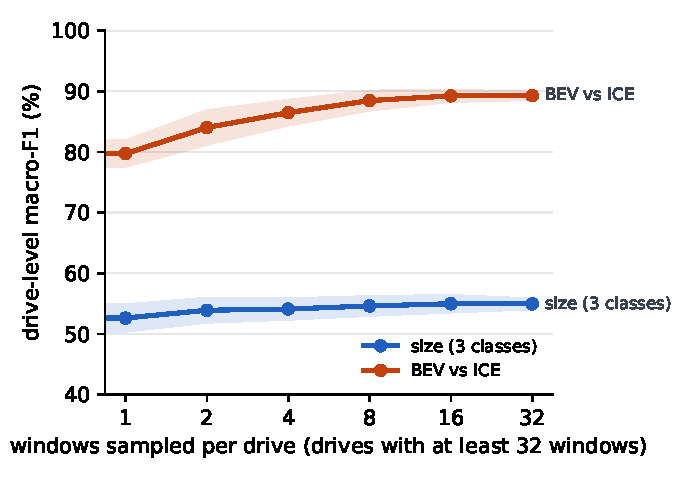
\includegraphics[width=0.85\columnwidth]{evidence_sufficiency.pdf}
\caption{Evidence sufficiency on held-out car models (reference predictions, drive-level macro-F1 in percent): on test drives with at least 32 eligible windows, $m$ windows are drawn per drive and their probability vectors averaged (mean over 50 draws; band: one std). Size moves from 52.6 ($m = 1$) to 54.9 ($m = 32$; all windows 56.0), BEV vs ICE from 79.7 to 89.3 (all windows 89.1), saturating by 8--16 windows.}
\label{fig:evidence}
\end{figure}

\subsection{Ceilings, Separability and Evidence Sufficiency}

Three zero-training oracles bound the size task on the held-out models: a per-car-model majority oracle (every drive of a held-out model gets that model's majority prediction) lifts the ensemble of the 12 reference deep runs from 63.2 to 72.0, so perfect within-model consistency would still leave size far from 90 (BEV vs ICE: 89.8 to 93.5). The footprint-noise oracle of Fig.~\ref{fig:ceiling} scores 92.1 at $\sigma = 0.10$ m$^2$ and 86.6 at 0.15, so reaching 90 needs a footprint error of about $\pm$0.12 m$^2$, about 2.5\% of a 4.6 m$^2$ footprint. A curb-mass oracle (two mass cuts fitted on the training drives) scores 63.3 on the 1,139 test drives with a known mass, so mass is no better proxy.

\begin{figure}[t]
\centering
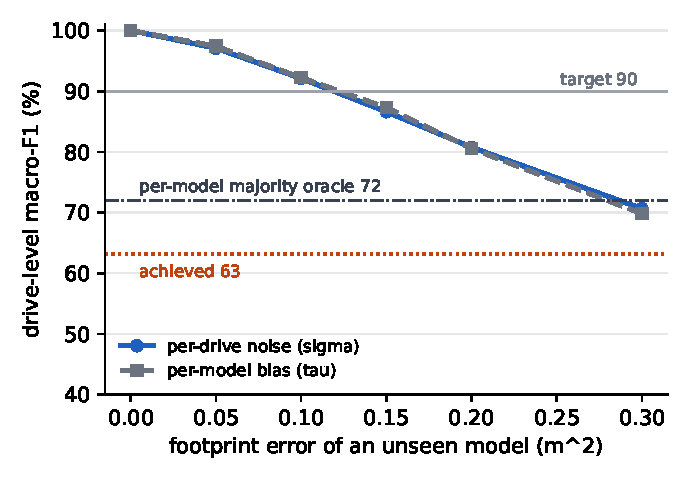
\includegraphics[width=0.85\columnwidth]{footprint_noise_oracle.pdf}
\caption{Footprint-noise oracle for the size task on held-out car models (drive-level macro-F1 in percent, 200 repeats): each drive is classified from the true footprint of its car model plus an error, cut at the fixed thresholds 4.43 and 4.88 m$^2$; per-drive noise of std $\sigma$ (circles) or a per-car-model bias $\tau$ (squares), both in m$^2$. Lines: the reference ensemble of the twelve reference sequence-model runs (63.2), its per-car-model majority oracle (72.0) and the 90 target.}
\label{fig:ceiling}
\end{figure}

The errors sit where the labels are closest: 21 of the 41 held-out car models lie within 0.15 m$^2$ of a differently labelled training model, and in one reference GRU run window accuracy is 53.0\% within 0.1 m$^2$ of a threshold against 89.9\% beyond 0.8 m$^2$. With the reference predictions, LARGE unibody vehicles are read as MID or SMALL while pickups and body-on-frame SUVs are recognised (per-model shares in Section~\ref{sec:discussion}), and MID models just above the 4.43 m$^2$ cut are read as SMALL (drives correct: GWM Haval H6, Audi Q5, Lexus RX and Nissan Altima 0\%, Kia Stinger 25\%).

Evidence per drive is not the limit for the reference models (Fig.~\ref{fig:evidence}): drive accuracy stays between 63.8 and 73.8\% (size) and 85.7 and 93.2\% (BEV vs ICE) from 1--2 to more than 64 windows per drive, and it does not grow with the number of acceleration, deceleration or lead-acceleration episodes.

\subsection{LLM-Proposed Physical Features}

Table~\ref{tab:llm} compares gradient boosting on hand-crafted window statistics, on the 34 registered LLM-proposed features and on both: alone, the physical features are weak per window but strong per drive, on a par with the reference sequence models on BEV vs ICE, and adding the statistics helps size but lowers BEV vs ICE at drive level. By permutation importance of the LLM-features-only gradient boosting on the validation split, BEV vs ICE rests on lift-off deceleration (while moving and shortly after pedal release), the share of deceleration under a pressed accelerator or without the brake, the lead-to-ego deceleration delay and the 10th percentile of brake-free deceleration; size on the curvature-per-steering-angle gain at 6--18 m/s and at low speed, the Ackermann gain at 6--12 m/s and the same delay.

\begin{table}[t]
\centering
\footnotesize
\setlength{\tabcolsep}{3.5pt}
\caption{Gradient boosting on window statistics, on the 34 registered LLM-proposed features and on both (held-out car models, one seed); macro-F1 in percent per window (full and human-only) and per drive (protocol full).}
\label{tab:llm}
\begin{tabular}{@{}lcccccc@{}}
\toprule
 & \multicolumn{3}{c}{Size} & \multicolumn{3}{c}{BEV vs ICE} \\
\cmidrule(lr){2-4} \cmidrule(lr){5-7}
Features & full & human & drive & full & human & drive \\
\midrule
Statistics & 49.7 & 46.3 & 54.7 & 69.5 & 73.5 & 73.2 \\
LLM physical & 40.5 & 47.3 & 63.2 & 69.6 & 84.2 & 89.4 \\
LLM + statistics & 54.1 & 49.8 & 64.9 & 73.2 & 80.2 & 80.9 \\
\bottomrule
\end{tabular}
\end{table}

\subsection{Aggregation and Ensembles}

Out of fold on the reference recipe (GRU and ResNet pooled), the best aggregation variant moves size from 67.5 to 67.8 (+0.3) and down-weighting DAS windows in the mean moves BEV vs ICE from 93.0 to 94.8 (+1.8), short of the pre-registered +1.0 on both tasks, so the plain mean remains the headline. Ensembles stayed below the G4 gate: a GRU + ResNet mean gains under one point over the best member out of fold (BEV vs ICE 93.9 against 93.1--93.5; size 68.8 against 68.2) and stacking is worse (92.3 and 66.5). The supplementary rule fixed before the final test run, the DAS- and episode-weighted log-odds mean of Section~\ref{sec:methods}, moves size from 66.9 to 68.7 on the six final S9 runs (+1.7, 6 of 6 runs improved) and BEV vs ICE from 92.8 to 93.5 on the six B5 runs (+0.7, 6 of 6).

\section{Discussion and Limitations}\label{sec:discussion}

\subsection{Label Resolution, Not Sensing}
Under the fixed footprint cut, 90 drive-level macro-F1 needs each held-out model's footprint to within about $\pm$0.12~m$^2$ (Fig.~\ref{fig:ceiling}). Two curb-mass cuts fitted on training models score only 63.3, and 21 of the 41 held-out car models lie within 0.15~m$^2$ of a differently labelled training model. The gap is set by label resolution and fleet composition, not by model capacity or evidence per drive: architectures stay within about 2 points (Table~\ref{tab:main}) and more windows per drive add little for size (Fig.~\ref{fig:evidence}). Per-model errors (Section~\ref{sec:experiments}) split LARGE by body type: pickups and body-on-frame SUVs are recognised (GMC Yukon, Ford Ranger and Ford F-150 Lightning: 95.5--100\% of drives), while unibody three-row SUVs and full-size sedans are read as MID or SMALL (Genesis G80 and G90, Volkswagen Atlas, Tesla Model~S and Kia EV9: 0--5.6\%), so the networks appear to learn LARGE as a truck's mass-and-driveline signature rather than as footprint.

\subsection{What 90 Needs}
Pooling a vehicle's drives does not rescue size (60.0--62.6 against 66.8--67.1 at drive level): about 45\% of the test vehicles have a single drive and the errors are per car model, so even the per-car-model majority oracle lifts the reference ensemble only from 63.2 to 72.0. Three routes remain: seen car models, as under held-out devices, where the same recipes reach 79.5--80.6 (Table~\ref{tab:device}); the vehicle level for BEV vs ICE, where the GRU B5 rises from 92.6 to 93.4 (95.5 on vehicles with at least two drives) and the ResNet B5 stays at 92.8--93.0; and labels whose margins exceed the resolution of about 0.12~m$^2$, such as cuts in wide gaps of the footprint distribution.

\subsection{Two Protocol Lessons}
First, while a driving automation system (DAS) is engaged, a controller tuned per car model supplies part of the control action. Windows with automation activity are easier for size than windows without (56.4 against 50.2, one bi-GRU run) and harder for BEV vs ICE (79.8 against 84.0, one ResNet B5 run): plausibly the controller carries platform information and masks the pedal behaviour that separates the powertrains. Hence the headline drive-level results (Table~\ref{tab:main}) are paired with the human-only protocol, and the final BEV vs ICE recipe (B5) down-weights DAS windows (the size variant S7 did not win in the fold-0 sweep, Table~\ref{tab:folds}). Second, early stopping on the released validation split, which shares car models with training, selects epochs 16--22, against 1--8 (median about 4) for the reference recipe on the model-disjoint folds (Section~\ref{sec:methods}), and the final models' validation scores do not predict their test scores (Section~\ref{sec:experiments}). Such a split rewards memorising car models, a shortcut~\cite{geirhos2020shortcut}; we therefore fixed the training length from the folds (Table~\ref{tab:folds}), and a future release would carve the validation split model-disjoint.

\subsection{Privacy and Limitations}
Section~\ref{sec:dataset} lists the privacy measures. Labels describe car models, not people: a rare model may be recognisable as a model, never as a person. The same property that makes the data useful, that motion reveals the vehicle, restricts access to research on vehicle dynamics and driving behaviour and prohibits re-identification and linkage with other datasets. Several limitations remain.
All logs come from one logger ecosystem and its software eras~\cite{schafer2018comma2k19}, and the fleet is skewed by region and brand (83.8\% of the hours from North America, 4.8\% from Europe, 4.2\% from Asia); region, software era and device type are metadata, not inputs, but they correlate with powertrain.
Labels are platform attributes: a misidentified platform mislabels every drive of that vehicle, and platforms sold with several powertrains the logs cannot separate, or of unknown powertrain, carry no powertrain label (11.1\% of the drives). On 56.2\% of the drives the lead vehicle comes from a camera model rather than a radar, and pedal magnitudes are missing on 63.9\% (accelerator) and 49.4\% (brake) of the drives. The internal folds never hold out the LARGE~$\times$~BEV cell, which one car model dominates, so their numbers for that cell reflect training models only; the test split does hold out models of that cell.
% Source of the fold statement: CAMPAIGN.md (G1/G2 consequence note) and INTERNAL_FOLDS.md (the LARGE x BEV pool is dominated by one car model); not in OUTLINE.md; verified 8 Nov 2026.
With 41 (size) and 39 (BEV vs ICE) test car models, the GRU recipes' cluster-bootstrap intervals are wide (67.1 [54.4, 74.2] and 92.6 [87.1, 96.2]); differences of a few points between methods lie inside them.

\section{Conclusion}\label{sec:conclusion}
We asked whether a vehicle's size class and powertrain can be read from 60-s windows of trajectory and CAN signals for car models never seen in training. The released dataset (9,062 drives, about 3,950 h, 1,431 pseudonymous vehicles, 174 car models) fixes the labels, the model-disjoint and device-disjoint splits, the window-, drive- and vehicle-level protocols and the cluster-bootstrap intervals over car models. Powertrain is readable: BEV vs ICE reaches 92.6--93.0 drive-level macro-F1 on held-out car models. Size under a footprint cut is only partly readable: a pre-registered campaign raised the bi-GRU drive-level score from 62.9 to 67.1 (point estimates whose bootstrap intervals overlap), four sequence architectures stay within about 2 points, and zero-training oracles show that 90 would need a footprint resolution of about $\pm$0.12~m$^2$, while half of the held-out car models lie within 0.15~m$^2$ of a differently labelled training model. These results are reference points, not a leaderboard. The next steps are labels with margins above that resolution, more fleets and car models, and vehicle-level evaluation where vehicles have several drives.


\ifanonymous\else
\section*{Acknowledgments}
% TODO (authors): funding and acknowledgments, or remove.
\fi

\bibliographystyle{IEEEtran}
\bibliography{refs}

\end{document}
"
\ifdefined\withauthors\anonymousfalse\else\anonymoustrue\fi

\ifanonymous
\author{\parbox{\textwidth}{\centering Author names withheld for review}}
\else
\author{%
	\parbox{\textwidth}{%
		\centering
		Yuhang Wang, Yuechen Guo, Jingxin Yang, Chuheng Wei, Suyang Chen,\\
		Abdulaziz Alhuraish, Yiyi Wang, Jingran Sun and Hao Zhou%
	}%
	% TODO (authors): affiliations and contact e-mails, e.g.
	% \thanks{$^{1}$Affiliation 1, City, Country {\tt\small contact address}}
}
\fi

\begin{document}
\maketitle
\thispagestyle{empty}
\pagestyle{empty}

\begin{abstract}
Trajectory data for traffic analytics, simulation calibration and infrastructure studies rarely record the vehicle type. We ask whether it can be read from motion alone: can 60-s windows of trajectory and CAN signals reveal the size class (three footprint classes) and the powertrain (battery-electric vs combustion, BEV vs ICE) of car models never seen in training? We release a pseudonymous dataset of 9,062 drives (about 3,950 h) from 1,431 vehicles and 174 car models, with held-out-car-model and held-out-device splits, window-, drive- and vehicle-level protocols and cluster-bootstrap intervals over car models. Four sequence architectures (ResNet, bi-GRU, Transformer, Mamba-2), hand-crafted statistics and physical features proposed by large language models (LLMs) serve as reference points; a pre-registered method study on model-disjoint internal folds adds car-model-balanced sampling, auxiliary physical targets, physics-safe augmentation, per-car-model loss re-weighting and, for BEV vs ICE, down-weighting of driving automation system (DAS) periods. On held-out car models, BEV vs ICE reaches 92.6--93.0 drive-level macro-F1 (95\% interval [87.1, 96.2] for the final bi-GRU); size improves from 62.9 to 67.1 at drive level but stays far from 90. Run unchanged on a public fleet of 4,061 devices absent from our library, the final models call the powertrain right for 86 of 88 car models and match the internal size result (63.2\% of devices against 63.5\% at vehicle level). Zero-training oracle analyses attribute the gap to label resolution and training-fleet composition rather than to evidence per drive; the architecture benchmark shows model capacity is not the bottleneck.
\end{abstract}
% W1: shorter title alternative, if wanted:
% "Reading Vehicle Size and Powertrain from Motion: A Trajectory--CAN Benchmark with Held-Out Car Models"

\section{Introduction}\label{sec:intro}

Vehicle trajectories are collected at scale by roadside sensors, connected-vehicle platforms and aftermarket loggers, usually without a reliable record of the vehicle that produced them. Many uses need it: traffic analytics by vehicle class, calibration of microscopic simulation models whose car-following parameters differ between a compact car and a three-row SUV, and infrastructure studies of how often heavy or electric vehicles use a facility. Registration records, licence plates or camera images can fill the gap but raise privacy and availability problems; a trajectory that reveals its vehicle type by itself would be more privacy-friendly.

Motion should carry this information: wheelbase, steering ratio and mass distribution set the yaw and curvature response to steering, and the powertrain shapes launches and lift-off deceleration, so a battery-electric vehicle (BEV) braking largely through its motor should leave a different speed trace from an internal-combustion-engine (ICE) vehicle. We pose the question as it arises in deployment, for car models never seen in training, since otherwise every new model would need retraining. From 60-s windows of trajectory and controller area network (CAN) signals (among them speed, acceleration, steering, yaw rate, curvature, lateral acceleration, pedal and automation flags, and lead-vehicle distance, relative speed, headway and time-to-collision; Section~\ref{sec:dataset} lists all channels) we predict a size class (SMALL, MID or LARGE, cut from the vehicle footprint) and the powertrain (BEV vs ICE).

Three things make this hard. First, the size label is a hard cut through a continuous quantity (footprints of 4.43 and 4.88 m$^2$ separate the classes), so a car model near a cut is hard to place even when its physics is read well. Second, a driving automation system (DAS) is engaged in 47.9\%
of the samples, so part of the measured behaviour is a controller signature that may not transfer between car models. Third, the fleet is uneven (174 car models from 38 brands with widely differing hours), so a held-out model in a footprint gap of the training fleet has no neighbour to be read against.

We therefore release the data with fixed labels and splits, benchmark sequence models and feature pipelines under one protocol, run a pre-registered method study on model-disjoint folds, and ask, without training anything, where the size ceiling lies and why. The contributions are:

\begin{itemize}
\item A public, privacy-preserving trajectory and CAN dataset (9,062 drives, about 3,950 h, 1,431 pseudonymous vehicles) with fixed footprint-size and powertrain labels, held-out-car-model (headline) and held-out-device splits, and window-, drive- and vehicle-level protocols with cluster-bootstrap intervals over car models (Section~\ref{sec:dataset}).
\item A benchmark of four sequence architectures, hand-crafted statistics and physical features proposed by a large language model (LLM) under those protocols, showing that architecture is not the bottleneck (all deep models within about 2 points) and drive-level aggregation adds 7--12 points (Table~\ref{tab:main}).
\item A pre-registered method study on model-disjoint internal folds (Sections~\ref{sec:methods} and \ref{sec:experiments}): car-model-balanced sampling, auxiliary physical targets, physics-safe augmentation, per-car-model loss re-weighting (size) and DAS down-weighting (BEV vs ICE) raise the drive-level result by 4--6 points (size) and 2--4 points (BEV vs ICE); an episode-centric multiple-instance model over driving transients matches but does not beat the window recipes on the test models.
\item Zero-training ceiling analyses (per-car-model majority, footprint-noise and curb-mass oracles, evidence sufficiency, separability of held-out models) that quantify why size cannot reach 90 on unseen car models under a footprint cut, and what would make it reachable (Figs.~\ref{fig:evidence} and \ref{fig:ceiling}).
\end{itemize}

\section{Related Work}\label{sec:related}

\textbf{Electric and combustion vehicles on the road.} Battery-electric vehicles accelerate and slow down differently from combustion vehicles: torque is available from standstill, much of the deceleration comes from regenerative rather than friction braking, and one-pedal driving lets the car decelerate strongly when the accelerator is released. Instrumented and naturalistic studies report such differences: drivers new to electric vehicles accelerate and brake differently at first and adapt over months~\cite{helmbrecht2014ev}, electric vehicles under adaptive cruise control follow with smoother speed profiles and shorter spacing than combustion vehicles~\cite{geffen2026ev}, and car-following models for electric vehicles add phases for strong acceleration and regenerative braking~\cite{liu2025paai}.
% TODO cite own EV-vs-ICE acceleration paper when citable (neutral phrasing for double-blind review)
Most of this work compares populations whose type is known; we ask the inverse question, whether the type can be recovered from the motion of a car model never observed in training.

\textbf{Vehicle and driver identification from kinematics and CAN.} Vehicle classification from GPS trajectories separates passenger cars from trucks with hand-crafted features~\cite{sun2013gps} or convolutional networks~\cite{dabiri2020gps}, and driver identification from CAN signals has shown that steering, pedal and speed traces carry strong identity information, from whole drives~\cite{enev2016fingerprinting} down to a single turn~\cite{hallac2016turn}. When such pipelines feed summary statistics to a tree ensemble~\cite{breiman2001rf,ke2017lightgbm} or a small network and split windows or trips at random, the same vehicles or car models appear on both sides, so identity rather than type may be learnt. Our splits hold out car models or devices by construction.

\textbf{Sequence models for time-series classification.} One-dimensional residual networks remain strong baselines for time-series classification~\cite{wang2017tsc,ismailfawaz2019review}; gated recurrent units~\cite{cho2014gru} and Transformer encoders~\cite{vaswani2017attention} are the usual recurrent and attention-based alternatives, and selective state-space models~\cite{gu2023mamba} with the structured state-space duality of Mamba-2~\cite{dao2024mamba2} offer linear-time sequence mixing. We benchmark one representative of each family under one protocol.

\textbf{Shortcut learning and group-disjoint evaluation.} Deep networks readily pick up cues that correlate with the label in training but not in deployment~\cite{geirhos2020shortcut}. For vehicle-type inference the obvious shortcuts are the identities of the car model and of the logging device, so we evaluate on held-out car models and report cluster-bootstrap intervals over models. Group distributionally robust optimisation~\cite{sagawa2020dro} and domain-adversarial training~\cite{ganin2016dann} are standard remedies for group shift; we test light-weight variants of both on model-disjoint internal folds.

\textbf{Multiple-instance learning and ordinal targets.} A drive is a bag of windows or episodes with a single label, which is the setting of attention-based multiple-instance learning~\cite{ilse2018mil}. The size classes are ordered cuts of a continuous footprint, so rank-consistent ordinal regression~\cite{cao2020coral} and direct regression of the footprint are natural auxiliary targets.

\textbf{Language models for time series and feature discovery.} Using large language models directly as time-series forecasters has been questioned~\cite{tan2024llmts}, while letting them propose programs that are then checked by execution has been fruitful~\cite{romeraparedes2024funsearch}. We follow the second route: agents propose physically motivated features as code, which verifiers and an auditor screen before they enter a standard classifier.

\textbf{Source logs.} The drives come from the open-source driving automation system (DAS) ecosystem behind comma2k19~\cite{schafer2018comma2k19} and a large-scale naturalistic take-over dataset~\cite{wang2026adasto}; we expose only vehicle-state and lead-vehicle signals under pseudonyms, without positions, absolute times or video (Section~\ref{sec:dataset}).

\section{Dataset and Protocols}
\label{sec:dataset}

\subsection{Source and Extraction}
The drives are open logs of vehicles running an open-source driving automation system (DAS), the ecosystem behind comma2k19~\cite{schafer2018comma2k19} and the take-over dataset of~\cite{wang2026adasto}. Drive tables are indexed by the 10~Hz vehicle-state sample (row $k$ at nominal time $k/10$~s). Lower-rate radar, pose and controller topics are zero-order held causally onto these sample times, with stale samples set to missing, and a flag marks rows preceded by a gap longer than 0.3~s. DAS-engaged periods are kept and flagged, so the same vehicles appear under human and automated driving.

\subsection{Channels}
Of the 44 columns of a drive table, 20 are the official model inputs: speed and longitudinal acceleration; steering-wheel angle, rate and normalised torque; yaw rate, curvature and lateral acceleration; the flags accelerator pressed, brake pressed, steering pressed, standstill and DAS engaged; and lead-vehicle validity, distance, relative speed, speed, acceleration (a causal slope of its speed), time headway and time to collision. Steering torque is normalised per drive by the 95th percentile of its magnitude while moving and steering. Pedal magnitudes are missing on 63.9\% (accelerator) and 49.4\% (brake) of the drives, so only the always-valid pressed flags are inputs; on 56.2\% of the drives the lead comes from a camera model rather than a radar.

\subsection{Labels}
Both labels are attributes of the platform identified from the bus, not of a drive. Size is the footprint, wheelbase $\times$ mean track: SMALL below 4.43~m$^2$, MID from 4.43 up to 4.88~m$^2$, LARGE from 4.88~m$^2$. The thresholds were locked on the label inventory before any classifier was trained: every size $\times$ \{BEV, ICE\} cell had to hold at least 100~h, 3 car models and 5 identity groups (same device, same vehicle identity or shared drive names); the admissible pairs maximising the smallest cell (309~h) were kept, each cut placed in a gap between platform footprints. Examples are the Civic and Bolt (SMALL), Camry and Model~3 (MID), Palisade and Model~X (LARGE); in that inventory the BEV hours of SMALL, MID and LARGE came from only 15, 10 and 8 car models, against 55, 42 and 28 for ICE. Powertrain is ICE, hybrid (HEV), plug-in hybrid (PHEV) or BEV, with BEV vs ICE the main task; platforms sold with several powertrains that the logs cannot separate (MIXED) or of unknown powertrain carry a null label (11.1\% of the drives). Table~\ref{tab:dataset} summarises the release.

\begin{table}[t]
\caption{Release summary. Vehicles are device $\times$ platform pairs; class support counts eligible 60-s windows; the test-split block counts eligible windows and the units they cover.}
\label{tab:dataset}
\centering
\footnotesize
\setlength{\tabcolsep}{4pt}
\begin{tabular}{@{}lr@{}}
\toprule
Drives (one ignition cycle each) & 9,062 \\
Hours, nominal & 3,949.8 \\
Hours moving & 3,078.1 \\
Pseudonymous vehicles & 1,431 \\
Identity groups (unit of the splits) & 1,157 \\
Platforms / brands / car models & 360 / 38 / 174 \\
Samples with DAS engaged & 47.9\% \\
Samples with any automation activity & 62.6\% \\
\midrule
Windows listed & 241,476 \\
Windows eligible & 201,390 \\
Windows human-only (strict) & 37,942 \\
Eligible windows, size & 201,169 \\
Eligible windows, BEV vs ICE & 144,534 \\
Eligible windows, four-class powertrain & 178,827 \\
\bottomrule
\end{tabular}

\vspace{0.5ex}

\begin{tabular}{@{}lrrrr@{}}
\toprule
Class & Windows & Hours & Vehicles & Platforms \\
\midrule
SMALL & 91,369 & 1,522.8 & 673 & 169 \\
MID & 56,059 & 934.3 & 392 & 104 \\
LARGE & 53,741 & 895.7 & 295 & 76 \\
\addlinespace
ICE & 79,566 & 1,326.1 & 598 & 200 \\
HEV & 23,708 & 395.1 & 197 & 57 \\
PHEV & 10,585 & 176.4 & 68 & 21 \\
BEV & 64,968 & 1,082.8 & 366 & 71 \\
Powertrain null & 22,563 & 376.1 & 156 & 34 \\
\bottomrule
\end{tabular}

\vspace{0.5ex}

\begin{tabular}{@{}lrr@{}}
\toprule
Test split, held-out car models & Size & BEV vs ICE \\
\midrule
Eligible windows & 26,144 & 18,295 \\
Hours & 435.7 & 304.9 \\
Drives & 1,141 & 836 \\
Vehicles & 329 & 244 \\
Car models & 41 & 39 \\
\bottomrule
\end{tabular}
\end{table}

\subsection{Splits}
Both schemes split by identity group, since drives of one device are correlated. The headline scheme, \texttt{split\_platform}, holds out whole car models, about 15\% of the hours of each size $\times$ powertrain cell, as the test split (last block of Table~\ref{tab:dataset}); drives of a group that also drove a held-out model are excluded from every split. The validation split is carved group-disjoint from the remaining pool and shares 53 of its 56 car models with train, so only the test split is model-disjoint and a validation score rewards recognising a known car model (Section~\ref{sec:methods}). The secondary scheme, \texttt{split\_device}, assigns groups at random inside each cell (70 / 15 / 15\% of the hours) and shares car models across splits, so its test measures generalisation to unseen devices of known models; lab-owned devices are always in train.

\subsection{Protocols}
A 60-s window is eligible when it has 600 consecutive samples, no gap and at least 20\% of its samples moving. Window-level protocols score each eligible test window on its own: \texttt{test\_full} takes all of them (headline), \texttt{test\_balanced} a published class-balanced list, and \texttt{test\_human\_only} the windows with no automation activity inside or in the 10~s before them.

Unit-level protocols pool the same per-window probabilities: \texttt{drive\_full} averages the probability vectors of a drive's \texttt{test\_full} windows and takes the arg-max, \texttt{drive\_human\_only} does so over human-only windows, and \texttt{vehicle\_full} pools every window of all test drives of a vehicle; units without a selected window are excluded. The metric is macro-F1 over the classes present. Held-out car models are the replication unit, so 95\% intervals come from a cluster bootstrap over car models (1,000 resamples, seed 0): each resample draws car models with replacement and keeps every unit of a drawn model once.

\subsection{Shortcut Audits}
Two group-disjoint audits with simple classifiers look for shortcuts~\cite{geirhos2020shortcut}: nuisance metadata columns predict powertrain at 0.32 macro-F1 (chance 0.25) and size at 0.40 (chance 0.33), so they stay out of the inputs; window statistics of the official inputs predict brand at 0.02 (chance 0.03 over 38 brands) and platform at 0.00 but powertrain at 0.31 and size at 0.34: no detectable brand fingerprint and little class information under this audit.

\subsection{Privacy and Availability}
Vehicles, drives and groups carry random, independent pseudonyms drawn for this release only. The release holds no positions, absolute times or dates, video, images or driver-monitoring signals; region is a continent-level bucket and time is relative to the start of each drive. Access is gated to research on vehicle dynamics and driving behaviour and prohibits re-identification of vehicles or drivers and linkage with other datasets. The data, indexes, split lists, schema and checksums are public under CC BY 4.0 and the build, evaluation and experiment code under the MIT License\ifanonymous; the repository links are withheld for review.\else: \url{https://huggingface.co/datasets/HenryYHW/Vehicle_Power_Type_Trajectory_Dataset} and \url{https://github.com/WangYuHang-cmd/-Vehicle_Power_Type_Trajectory_Dataset}.\fi
% source: the access conditions, the continent-level region bucket, the absence of driver-monitoring signals and the licence names come from the dataset card, not from OUTLINE.md

\section{Methods}\label{sec:methods}
% length (W3, trim pass + second fixer pass): about 1,165 whitespace tokens of prose on non-comment lines against the 1,000-word budget (first draft 1,912, fixer pass 1,586, trim pass 1,082). Episode detection thresholds, augmentation probabilities, the reference learning rate, bag sizes, fold pool hours and the MIL training details are kept in comments next to the prose they belong to; restore any of them if space allows. Details that Section V states itself (seeds, the gated-attention ablation, permutation importance on the validation split) are not repeated here. The fold pool sizes stay in the comment under Part C.

All methods read only the 20 official channels of Section~\ref{sec:dataset} and quantities derived from them. Parts A--B and F are the first round, Parts C--E and G the pre-registered campaign.

\subsection{Window Models}

A window is a $600 \times 20$ array (60 s at 10 Hz), standardised per channel with training-split statistics. We compare four sequence classifiers \cite{wang2017tsc,ismailfawaz2019review}: a 1-D ResNet \cite{wang2017tsc} on the 10 Hz signal and three token models on a shared two-layer convolutional stem with stride 4 (150 tokens of width 128): two bidirectional GRU layers \cite{cho2014gru}, a four-layer Transformer encoder \cite{vaswani2017attention} and four bidirectional Mamba-2 layers \cite{gu2023mamba,dao2024mamba2}, a pure-PyTorch implementation of the published algorithm. All four share one pooling head whose hidden vector is the window embedding reused in Part E. Parameters: ResNet 2.31 M, bi-GRU 0.73 M, Transformer 0.70 M, Mamba-2 1.07 M.
% inputs clipped, missing values set to 0; Mamba-2 block = the chunked state-space-duality scan run forward and on the reversed tokens, without custom kernels

\subsection{Reference Training Recipe}

Training uses class-balanced sampling weights $(N / (K n_k))^{0.5}$ capped at 10 ($N$ windows, $K$ classes, $n_k$ per class), AdamW \cite{loshchilov2019adamw} with warm-up over the first 3\%
of the steps and cosine decay, batches of 256, label smoothing 0.05 and early stopping on validation window macro-F1. The feature baselines feed 180 window statistics (nine per channel) and the physical features proposed by large language models (LLMs) in Part F to a class-balanced logistic regression and a histogram gradient-boosting classifier \cite{pedregosa2011sklearn,ke2017lightgbm}.
% at most 25 epochs, patience 6; learning rate 1e-3 (5e-4 for the Transformer) and weight decay 0.05 (experiments/train.py DEFAULTS and LR_BY_MODEL; not in OUTLINE.md); statistics = moments, extremes, quantiles, roughness and coverage; features and statistics are evaluated alone and together, under the same splits and protocols; seeds are stated in Section V

\subsection{Model-Disjoint Internal Folds and Pre-Registration}

Because the released validation split shares car models with training (Section~\ref{sec:dataset}), every campaign choice was made on internal car-model-disjoint folds drawn per task from the train + validation pool: three folds per task hold out 19 of 57 candidate car models (size) and 16, 15 and 20 (BEV vs ICE). A fold's training set drops every drive whose identity group also drove a held-out model; the one shared device pool spanning 19 car models is not an owner and loses only its drives of held-out models (fleet rule).
% pools (OUTLINE.md): size 168,588 windows, 2,810 h, 117 car models; BEV vs ICE 121,381 windows, 2,023 h, 107 car models; fleet group = 33 vehicles, about 480 h, 13.3 % of the size pool's windows

For the reference recipe, early stopping on the shared-model validation split selects epochs 16--22, on the folds 1--8 (median about 4): that validation rewards memorising car models. Final models therefore train for the median fold best epoch (GRU S9 11, ResNet S9 16, GRU B5 2, ResNet B5 7, episode model 10).
% the validation split is only reported (Section V)

Six gates were pre-registered; G0 and G5 are procedural (stored numbers reproduced; one frozen test read per final model). G1: the reference recipe's fold drive-level score lies within 5 points of its test value, else the folds would have been redesigned. G2: the best recipe reaches a fold floor of 70 (size) or, for BEV vs ICE, 90 and at least 1 point over the reference recipe (or 92 on human-only drives); on failure, size reports ceilings instead of a 90 target and BEV vs ICE keeps the reference recipe. G3: the episode model gains 2 points over the best window recipe (size) or reaches 91 (BEV vs ICE), else it is only an ablation. G4: an ensemble or stacker needs 1.0 points over the best single model out of fold (outcomes in Section~\ref{sec:experiments} and Table~\ref{tab:folds}).

\subsection{Recipe Changes S1--S9 and B1--B5}

Each ladder adds one change at a time to the reference S0 / B0 (S1--S6 cumulative, S7--S9 each on S5; the BEV-vs-ICE ladder skips S3 and S6). S1 / B1: car-model-balanced sampling inside each class (shares $\propto$ hours$^{0.5}$). S2 / B2: regression head on the log footprint. S3: CORAL ordinal head \cite{cao2020coral}. S4 / B3: log curb-mass and four-class powertrain heads (B3 also trains the auxiliary heads on HEV / PHEV windows). S5 / B4: physics-safe augmentation (joint sign flip of the six lateral channels, one masked 3--15 s span with the lead validity flag cleared, dropout of one channel group, Gaussian noise 0.02). S6: same-class cutmix across car models. S7 / B5: down-weighting of windows with driving automation system (DAS) activity by $(1 - \beta) + \beta (1 - s)$, $s$ the DAS share, $\beta = 0.5$. S8: conditional adversarial car-model head \cite{ganin2016dann,long2018cdan} with gradient reversal ($\lambda = 0.1$). S9: group-DRO-lite \cite{sagawa2020dro} (per-car-model loss re-weighting). Decisions stay softmax arg-max; the final recipes are S9 (size) and B5 (BEV vs ICE).
% augmentation details (OUTLINE.md): sign flip p 0.5, masked span p 0.5, channel groups = lead / steering torque / pedals with p 0.1; no speed or amplitude scaling and no time reversal (both change the vehicle signature); heads: SmoothL1 on the standardised log footprint; loss weights classification 1, CORAL 0.5, footprint 1, mass 0.5, powertrain-4 0.3; S9 weights = softmax over running per-car-model losses

\subsection{Episode-Centric Multiple-Instance Model}

The episode MIL (multiple-instance learning) model treats each drive as a bag of the transients in which mass and powertrain should show, trained for both tasks jointly. Eight episode types are detected on Savitzky-Golay-smoothed speed \cite{savitzky1964}: ACC (acceleration), DEC\_LIFT and DEC\_BRK (deceleration with the brake mostly released or pressed), STOP, LAUNCH, LEAD\_ACC and LEAD\_DEC (lead acceleration or deceleration onsets in car-following range) and TURN (sustained low-speed curvature); 735,571 episodes come from 8,662 drives (545 have none). An episode is an 18-s onset-anchored crop of 22 channels (the 20 inputs, smoothed acceleration, validity) with a 9-dimensional context vector; acceleration and deceleration episodes are also re-indexed on a speed grid (0--36 m/s, 0.5 m/s bins) as an acceleration-against-speed profile $a(v)$.
% detection thresholds left out for length (OUTLINE.md, Episodes and the MIL model): filter 5 samples / order 2; ACC / DEC = monotone segments (tolerance 0.3 m/s) of >= 3 s with |dv| >= 2 m/s and mean |a| >= 0.1 m/s^2, 2 s of cruise trimmed at both ends; DEC_LIFT = brake pressed in <= 10 % of the samples; STOP = standstill >= 1 s reached from >= 2 m/s within 15 s; LAUNCH = departure from standstill; LEAD_ACC / LEAD_DEC = lead slope >= 0.5 / <= -0.6 m/s^2 held 1 s after 2 s below 0.3 m/s^2 in car-following range (headway <= 6 s), ego response a >= 0.3 m/s^2 for 0.5 s within 8 s; TURN = |curvature| >= 0.01 1/m for >= 1 s at 2-12 m/s
% representation details left out for length (OUTLINE.md): context = anchor speed, speed change, duration, mean and peak acceleration, automation share, lead share, headway, gap flag; 180 stored samples, onset at sample 40 (STOP: standstill onset at sample 140); grid = 72 bins x 6 channels (smoothed acceleration, pedal flags, automation flag, validity, time from onset)

A shared encoder ($d = 128$; convolutional stem, residual blocks, type embedding, context MLP) embeds the crops, a grid encoder the $a(v)$ grid, and an adapter the frozen 60-s window embeddings of the window models (Part A) as a ninth instance type; on the folds the adapter uses only the fold's own window checkpoints. Gated attention \cite{ilse2018mil} pools each bag per task; heads predict size, BEV vs ICE, four-class powertrain, log footprint, log curb mass and two ordinal thresholds. The loss is the bag cross-entropies + 0.3 instance cross-entropies + 0.5 Huber(log footprint) + 0.25 Huber(log mass) + 0.25 cross-entropy (powertrain-4) + 0.25 binary cross-entropy (ordinal); about 0.99 M parameters train for a fixed 10 epochs (AdamW, warm-up, cosine decay). The bag prediction is the drive-level output; window-mean aggregation of the same model gives the row comparable with the window recipes.
% training details (OUTLINE.md unless marked): bag cross-entropies with label smoothing 0.05, masked by task eligibility; bags of up to 64 episodes (lead and turn episodes first, each capped at 16) + 8 window embeddings per drive in training, 128 + 16 at evaluation; batches of 24 drives with a cap on the share of one car model (code: 10 %, not in OUTLINE.md); augmentation = lateral sign flip p 0.5, instance dropout 0.2, lead dropout 0.1, noise 0.02, crop jitter (code: 160 of the 180 stored samples, offset 10 at evaluation, jitter 0-20 samples; not in OUTLINE.md); learning rate 1e-3 and weight decay 0.05 (experiments/mil_train.py DEFAULTS); the gated-attention vs learned-mean ablation is reported in Section V

\subsection{LLM-Assisted Feature Discovery}

Following Section~\ref{sec:related}, LLMs only propose programs that a verifier scores \cite{romeraparedes2024funsearch}; they never classify. Six proposer agents, one physics lens each, saw the channel definitions and a training-only sample of 2,727 windows and proposed 74 candidate features; six verifier agents ran the code, measured class separation and dropped 21, and an auditor removed 19 more, leaving 34 registered features. The coverage floor (the minimum share of windows on which a feature is defined) was lowered from 40\% to 10\%
because gradient boosting treats a missing regime as information; everything was fixed before any evaluation split was touched.
% pipeline details (OUTLINE.md): lenses = longitudinal powertrain, transmission signature, braking / regeneration / coasting, lateral inertia and geometry, car-following interaction, speed-dependent capability; 62 features + 12 from a gap-filling round; verifiers dropped 21 (coverage below the floor, degenerate or duplicate); the auditor's 19 = 6 in the first audit + 13 in the second (duplicates, a v^2 speed confound, controller-driven cues such as lead-response gain and lag and braking-onset time-to-collision, recording artefacts); the first pass with the 40 % floor let 12 features reach the auditor, the 10 % floor re-admitted 29; permutation importance is measured on the validation split (Section V)

\subsection{Aggregation to Drive and Vehicle Level}

Drive and vehicle protocols are those of Section~\ref{sec:dataset} (mean of the per-window probability vectors, arg-max). Out of fold, weighted (DAS, episode, steering) arithmetic and log-odds means, robust and gated means and a two-stage vehicle rule were compared with the plain mean on the reference recipe; none gained the required 1.0 drive-level points on both tasks (Section~\ref{sec:experiments}). A supplementary rule fixed before the final test run, the log-odds mean with window weights $(1 - s + 0.1)^{0.5} \times (1 + n_{\mathrm{acc}} + n_{\mathrm{dec}})$ ($s$ DAS share, $n$ acceleration / deceleration episode counts), is reported beside every final model.

\section{Experiments}\label{sec:experiments}

\subsection{Set-Up}

All runs used one RTX 5080 GPU (16 GB). Seeds are stated in the table captions; the gradient-boosting baselines (GBM) use scikit-learn~\cite{pedregosa2011sklearn}. Macro-F1 is in percent under the protocols of Section~\ref{sec:dataset}; the headline is the drive level on held-out car models, scored once per final model after all choices had been made on the internal folds. Unit-level intervals are 95\% cluster bootstraps over car models (with several seeds, the mean of the seeds' bounds); multi-seed entries are mean $\pm$ std.

\subsection{Main Results on Held-Out Car Models}

Table~\ref{tab:main} gives the headline results. Architecture is not the bottleneck: the four reference sequence models lie within about 2 points at window level and close together at drive level. Averaging the windows of a drive adds 7--12 points; pooling further to vehicle level does not. For the sequence models, windows without automation activity (human-only columns) are harder for size and easier for BEV vs ICE, which Section~\ref{sec:discussion} relates to the controller of the driving automation system (DAS); the human-only drive columns cover fewer drives and are not directly comparable with the full columns.

\begin{table*}[t]
\centering
\footnotesize
\setlength{\tabcolsep}{3.2pt}
\caption{Held-out car models (\texttt{split\_platform} test split; size / BEV vs ICE: 41 / 39 car models, 1,141 / 836 drives, 732 / 564 with human-only windows, 329 / 244 vehicles). Macro-F1 in percent (protocols of Section~\ref{sec:dataset}); deep models mean over three seeds (std where given), GBM single-seed; chance about 33 (size) and 50 (BEV vs ICE). S9 / B5: recipes selected on the internal folds (Section~\ref{sec:methods}); episode MIL with window-mean aggregation and its own bag prediction; bootstrap intervals in the text.}
\label{tab:main}
\begin{tabular}{@{}lcccccccccc@{}}
\toprule
 & \multicolumn{5}{c}{Size (SMALL / MID / LARGE)} & \multicolumn{5}{c}{BEV vs ICE} \\
\cmidrule(lr){2-6} \cmidrule(lr){7-11}
 & \multicolumn{2}{c}{window} & \multicolumn{2}{c}{drive} & vehicle & \multicolumn{2}{c}{window} & \multicolumn{2}{c}{drive} & vehicle \\
\cmidrule(lr){2-3} \cmidrule(lr){4-5} \cmidrule(lr){6-6} \cmidrule(lr){7-8} \cmidrule(lr){9-10} \cmidrule(lr){11-11}
Model & full & human & full & human & full & full & human & full & human & full \\
\midrule
Statistics + GBM & 49.7 & 46.3 & 54.7 & 50.5 & 51.5 & 69.5 & 73.5 & 73.2 & 74.3 & 76.0 \\
LLM features + GBM & 40.5 & 47.3 & 63.2 & 58.9 & 58.6 & 69.6 & 84.2 & 89.4 & 89.1 & 90.1 \\
LLM + statistics + GBM & 54.1 & 49.8 & 64.9 & 64.2 & 61.8 & 73.2 & 80.2 & 80.9 & 82.6 & 83.4 \\
\midrule
1-D ResNet & 53.6 $\pm$ 1.0 & 48.0 & 61.1 $\pm$ 1.3 & 60.3 & 56.4 & 78.4 $\pm$ 0.4 & 83.2 & 91.1 $\pm$ 0.8 & 89.5 & 90.3 \\
bi-GRU & 54.7 $\pm$ 0.3 & 50.4 & 62.9 $\pm$ 0.8 & 63.3 & 57.2 & 79.2 $\pm$ 0.8 & 85.2 & 89.0 $\pm$ 0.1 & 90.8 & 88.6 \\
Transformer & 52.5 $\pm$ 0.8 & 47.7 & 61.8 $\pm$ 0.9 & 61.3 & 55.3 & 77.0 $\pm$ 0.4 & 83.5 & 88.4 $\pm$ 0.6 & 90.1 & 89.0 \\
Mamba-2 (bidirectional) & 53.1 $\pm$ 0.4 & 49.8 & 61.2 $\pm$ 0.3 & 61.1 & 55.2 & 77.3 $\pm$ 0.7 & 84.0 & 89.4 $\pm$ 0.3 & 90.9 & 90.6 \\
\midrule
bi-GRU, S9 & 53.2 $\pm$ 0.3 & 47.8 & 67.1 $\pm$ 0.0 & 61.7 & 60.0 $\pm$ 0.6 & -- & -- & -- & -- & -- \\
1-D ResNet, S9 & 53.2 $\pm$ 0.8 & 49.5 & 66.8 $\pm$ 1.7 & 62.9 & 62.6 $\pm$ 1.4 & -- & -- & -- & -- & -- \\
bi-GRU, B5 & -- & -- & -- & -- & -- & 77.0 $\pm$ 0.3 & 83.7 & 92.6 $\pm$ 0.1 & 89.1 & 93.4 $\pm$ 0.4 \\
1-D ResNet, B5 & -- & -- & -- & -- & -- & 79.9 $\pm$ 0.7 & 83.2 & 93.0 $\pm$ 0.8 & 88.7 & 92.8 $\pm$ 0.4 \\
Episode MIL, window mean & 54.2 $\pm$ 0.3 & 50.0 & 64.6 $\pm$ 0.5 & 62.5 & 62.3 $\pm$ 0.9 & 78.8 $\pm$ 0.1 & 82.2 & 90.2 $\pm$ 0.2 & 89.9 & 90.4 $\pm$ 0.5 \\
Episode MIL, bag prediction & -- & -- & 64.3 & 63.2 & 62.4 & -- & -- & 93.0 & 91.5 & 92.8 \\
\bottomrule
\end{tabular}
\end{table*}

The recipes selected on the folds raise the drive level without a matching gain at window level: S9 adds 4--6 points on size and B5 2--4 points on BEV vs ICE over the reference GRU and ResNet. The gains are stable over seeds, but the intervals over car models overlap (GRU S9 67.1 [54.4, 74.2] against the reference GRU 62.9 [48.9, 72.4]; GRU B5 92.6 [87.1, 96.2] against 89.0 [81.8, 93.7]). The episode MIL model matches but does not beat the window recipes under either aggregation; its fold advantage on BEV vs ICE (95.8, Table~\ref{tab:folds}) did not carry to the test models.

\subsection{Held-Out Devices}

Table~\ref{tab:device} repeats the main rows with devices held out and car models shared: all drive-level scores are far higher and the LLM + statistics GBM becomes the best size model. The recipes appear to trade within-model recognition for cross-model generalisation, since GRU S9 is below the reference GRU at window level and slightly above it at drive level (79.5 [70.8, 84.4] against 78.1).

\begin{table}[t]
\centering
\footnotesize
\setlength{\tabcolsep}{3pt}
\caption{Held-out devices, car models shared (\texttt{split\_device} test split; size 1,218 drives / 219 vehicles / 81 car models, BEV vs ICE 922 / 143 / 63). Macro-F1 in percent per window and per drive (protocol full); mean $\pm$ std over three seeds, one seed for GBM and MIL.}
\label{tab:device}
\begin{tabular}{@{}lcccc@{}}
\toprule
 & \multicolumn{2}{c}{Size} & \multicolumn{2}{c}{BEV vs ICE} \\
\cmidrule(lr){2-3} \cmidrule(lr){4-5}
Model & window & drive & window & drive \\
\midrule
LLM + stat. + GBM & 72.4 & 80.6 & 84.4 & 94.1 \\
1-D ResNet & 68.4 $\pm$ 3.0 & 77.4 $\pm$ 2.2 & 82.4 $\pm$ 0.7 & 96.2 $\pm$ 0.5 \\
bi-GRU & 70.2 $\pm$ 0.9 & 78.1 $\pm$ 1.4 & 87.4 $\pm$ 0.4 & 96.5 $\pm$ 0.1 \\
ResNet S9 / B5 & 64.8 $\pm$ 0.3 & 80.6 $\pm$ 0.1 & 83.1 $\pm$ 0.2 & 97.2 $\pm$ 0.3 \\
GRU S9 / B5 & 62.9 $\pm$ 1.0 & 79.5 $\pm$ 0.7 & 78.8 $\pm$ 0.4 & 95.1 $\pm$ 0.3 \\
MIL (1 seed) & 68.4 & 78.8 & 86.5 & 96.1 \\
\bottomrule
\end{tabular}
\end{table}

\subsection{Internal Folds and Recipe Sweep}

Table~\ref{tab:folds} summarises the campaign on the internal folds of Section~\ref{sec:methods}. Gate G1 passed: the three-fold means of the reference recipe lie within about 5 points of its test values in Table~\ref{tab:main}. The fold-0 size sweep spans 4 points, no more than the spread between folds, and no recipe approaches 70, so gate G2 for size fails; on BEV vs ICE, augmentation (B4) brings the gain and B5 reaches 93.1 over three folds, passing G2. The episode MIL model with gated attention~\cite{ilse2018mil} is level with S9 on size (G3 fails) and +2.7 over B5 on BEV vs ICE (G3 passes); its window-mean aggregation is weaker (61.1 and 88.8), and gated attention beats a learned instance mean on fold 0 (67.8 against 66.7; 96.0 against 94.8).

The final models train for fixed epoch counts taken from the folds; their shared-model validation scores (GRU / ResNet S9 60.7 / 62.8 and B5 75.6 / 79.3; MIL 79.1 on size and 97.5 on BEV vs ICE) are no guide to the test values.

\begin{table}[t]
\centering
\footnotesize
\caption{Model-disjoint internal folds of Section~\ref{sec:methods}: drive-level macro-F1 (protocol full) on each fold's held-out car models and the three-fold mean, one seed per entry; MIL rows are the model's own bag prediction; S0 / B0 reference, S9 / B5 final recipes. (a) Fold-0 sweep with the bi-GRU; (b) candidates on all three folds.}
\label{tab:folds}
\setlength{\tabcolsep}{2.3pt}
\begin{tabular}{@{}lcccccccccc@{}}
\toprule
\multicolumn{11}{@{}l}{(a) Fold 0, bi-GRU} \\
\midrule
Size & S0 & S1 & S2 & S3 & S4 & S5 & S6 & S7 & S8 & S9 \\
 & 65.3 & 62.8 & 66.8 & 64.8 & 65.2 & 66.2 & 64.8 & 65.6 & 66.5 & 66.9 \\
\addlinespace
BEV vs ICE & B0 & B1 & B2 & B3 & B4 & B5 & & & & \\
 & 89.4 & 88.0 & 87.4 & 88.7 & 92.8 & 92.8 & & & & \\
\bottomrule
\end{tabular}
\par\smallskip
\setlength{\tabcolsep}{4pt}
\begin{tabular}{@{}lcccc@{}}
\toprule
\multicolumn{5}{@{}l}{(b) Three folds} \\
\midrule
Recipe & fold 0 & fold 1 & fold 2 & mean \\
\midrule
\multicolumn{5}{@{}l}{\emph{Size}} \\
GRU S0 (reference) & 65.3 & 69.5 & 60.4 & 65.1 \\
GRU S2 (footprint head) & 66.8 & -- & -- & 65.5 \\
GRU S5 (augmentation) & 66.2 & -- & -- & 66.5 \\
GRU S9 (final) & 66.9 & 70.5 & 64.8 & 67.4 \\
ResNet S0 (reference) & -- & -- & -- & 66.6 \\
ResNet S9 (final) & 67.0 & 70.4 & 61.2 & 66.2 \\
Episode MIL, bag & 67.8 & 65.6 & 67.5 & 67.0 \\
\addlinespace
\multicolumn{5}{@{}l}{\emph{BEV vs ICE}} \\
GRU B0 (reference) & 89.4 & 90.8 & 95.4 & 91.9 \\
GRU B4 (augmentation) & 92.8 & -- & -- & 92.8 \\
GRU B5 (final) & 92.8 & 91.1 & 95.4 & 93.1 \\
ResNet B0 (reference) & -- & -- & -- & 93.1 \\
ResNet B5 (final) & 95.7 & 93.9 & 96.1 & 95.2 \\
Episode MIL, bag & 96.0 & 98.2 & 93.2 & 95.8 \\
\bottomrule
\end{tabular}
\end{table}

\begin{figure}[t]
\centering
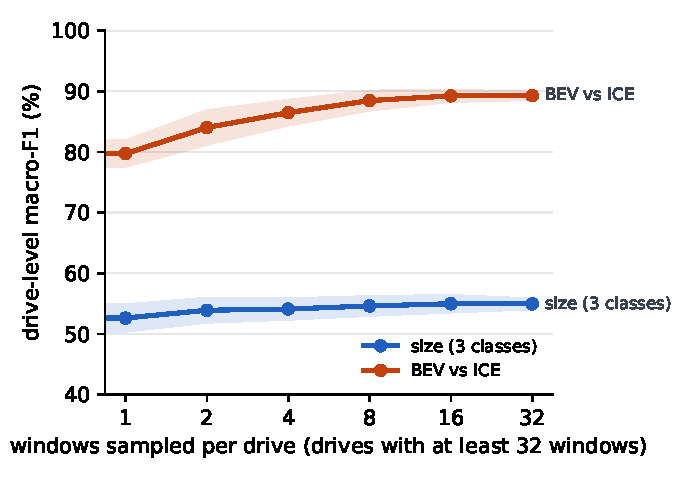
\includegraphics[width=0.85\columnwidth]{evidence_sufficiency.pdf}
\caption{Evidence sufficiency on held-out car models (reference predictions, drive-level macro-F1 in percent): on test drives with at least 32 eligible windows, $m$ windows are drawn per drive and their probability vectors averaged (mean over 50 draws; band: one std). Size moves from 52.6 ($m = 1$) to 54.9 ($m = 32$; all windows 56.0), BEV vs ICE from 79.7 to 89.3 (all windows 89.1), saturating by 8--16 windows.}
\label{fig:evidence}
\end{figure}

\subsection{Ceilings, Separability and Evidence Sufficiency}

Three zero-training oracles bound the size task on the held-out models: a per-car-model majority oracle (every drive of a held-out model gets that model's majority prediction) lifts the ensemble of the 12 reference deep runs from 63.2 to 72.0, so perfect within-model consistency would still leave size far from 90 (BEV vs ICE: 89.8 to 93.5). The footprint-noise oracle of Fig.~\ref{fig:ceiling} scores 92.1 at $\sigma = 0.10$ m$^2$ and 86.6 at 0.15, so reaching 90 needs a footprint error of about $\pm$0.12 m$^2$, about 2.5\% of a 4.6 m$^2$ footprint. A curb-mass oracle (two mass cuts fitted on the training drives) scores 63.3 on the 1,139 test drives with a known mass, so mass is no better proxy.

\begin{figure}[t]
\centering
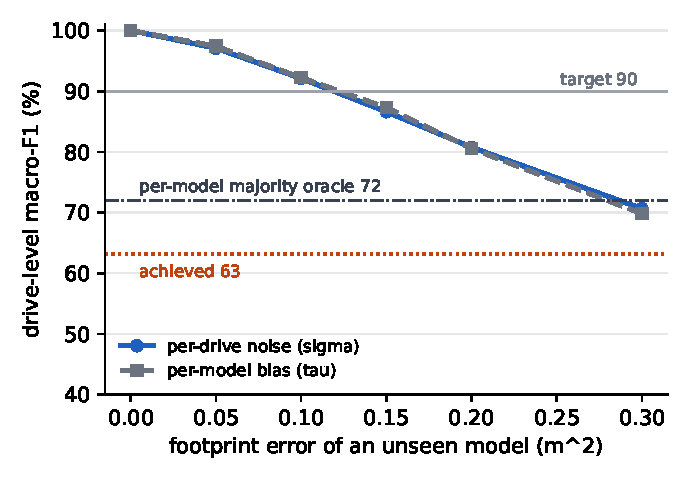
\includegraphics[width=0.85\columnwidth]{footprint_noise_oracle.pdf}
\caption{Footprint-noise oracle for the size task on held-out car models (drive-level macro-F1 in percent, 200 repeats): each drive is classified from the true footprint of its car model plus an error, cut at the fixed thresholds 4.43 and 4.88 m$^2$; per-drive noise of std $\sigma$ (circles) or a per-car-model bias $\tau$ (squares), both in m$^2$. Lines: the reference ensemble of the twelve reference sequence-model runs (63.2), its per-car-model majority oracle (72.0) and the 90 target.}
\label{fig:ceiling}
\end{figure}

The errors sit where the labels are closest: 21 of the 41 held-out car models lie within 0.15 m$^2$ of a differently labelled training model, and in one reference GRU run window accuracy is 53.0\% within 0.1 m$^2$ of a threshold against 89.9\% beyond 0.8 m$^2$. With the reference predictions, LARGE unibody vehicles are read as MID or SMALL while pickups and body-on-frame SUVs are recognised (per-model shares in Section~\ref{sec:discussion}), and MID models just above the 4.43 m$^2$ cut are read as SMALL (drives correct: GWM Haval H6, Audi Q5, Lexus RX and Nissan Altima 0\%, Kia Stinger 25\%).

Evidence per drive is not the limit for the reference models (Fig.~\ref{fig:evidence}): drive accuracy stays between 63.8 and 73.8\% (size) and 85.7 and 93.2\% (BEV vs ICE) from 1--2 to more than 64 windows per drive, and it does not grow with the number of acceleration, deceleration or lead-acceleration episodes.

\subsection{LLM-Proposed Physical Features}

Table~\ref{tab:llm} compares gradient boosting on hand-crafted window statistics, on the 34 registered LLM-proposed features and on both: alone, the physical features are weak per window but strong per drive, on a par with the reference sequence models on BEV vs ICE, and adding the statistics helps size but lowers BEV vs ICE at drive level. By permutation importance of the LLM-features-only gradient boosting on the validation split, BEV vs ICE rests on lift-off deceleration (while moving and shortly after pedal release), the share of deceleration under a pressed accelerator or without the brake, the lead-to-ego deceleration delay and the 10th percentile of brake-free deceleration; size on the curvature-per-steering-angle gain at 6--18 m/s and at low speed, the Ackermann gain at 6--12 m/s and the same delay.

\begin{table}[t]
\centering
\footnotesize
\setlength{\tabcolsep}{3.5pt}
\caption{Gradient boosting on window statistics, on the 34 registered LLM-proposed features and on both (held-out car models, one seed); macro-F1 in percent per window (full and human-only) and per drive (protocol full).}
\label{tab:llm}
\begin{tabular}{@{}lcccccc@{}}
\toprule
 & \multicolumn{3}{c}{Size} & \multicolumn{3}{c}{BEV vs ICE} \\
\cmidrule(lr){2-4} \cmidrule(lr){5-7}
Features & full & human & drive & full & human & drive \\
\midrule
Statistics & 49.7 & 46.3 & 54.7 & 69.5 & 73.5 & 73.2 \\
LLM physical & 40.5 & 47.3 & 63.2 & 69.6 & 84.2 & 89.4 \\
LLM + statistics & 54.1 & 49.8 & 64.9 & 73.2 & 80.2 & 80.9 \\
\bottomrule
\end{tabular}
\end{table}

\subsection{Aggregation and Ensembles}

Out of fold on the reference recipe (GRU and ResNet pooled), the best aggregation variant moves size from 67.5 to 67.8 (+0.3) and down-weighting DAS windows in the mean moves BEV vs ICE from 93.0 to 94.8 (+1.8), short of the pre-registered +1.0 on both tasks, so the plain mean remains the headline. Ensembles stayed below the G4 gate: a GRU + ResNet mean gains under one point over the best member out of fold (BEV vs ICE 93.9 against 93.1--93.5; size 68.8 against 68.2) and stacking is worse (92.3 and 66.5). The supplementary rule fixed before the final test run, the DAS- and episode-weighted log-odds mean of Section~\ref{sec:methods}, moves size from 66.9 to 68.7 on the six final S9 runs (+1.7, 6 of 6 runs improved) and BEV vs ICE from 92.8 to 93.5 on the six B5 runs (+0.7, 6 of 6).

\section{Discussion and Limitations}\label{sec:discussion}

\subsection{Label Resolution, Not Sensing}
Under the fixed footprint cut, 90 drive-level macro-F1 needs each held-out model's footprint to within about $\pm$0.12~m$^2$ (Fig.~\ref{fig:ceiling}). Two curb-mass cuts fitted on training models score only 63.3, and 21 of the 41 held-out car models lie within 0.15~m$^2$ of a differently labelled training model. The gap is set by label resolution and fleet composition, not by model capacity or evidence per drive: architectures stay within about 2 points (Table~\ref{tab:main}) and more windows per drive add little for size (Fig.~\ref{fig:evidence}). Per-model errors (Section~\ref{sec:experiments}) split LARGE by body type: pickups and body-on-frame SUVs are recognised (GMC Yukon, Ford Ranger and Ford F-150 Lightning: 95.5--100\% of drives), while unibody three-row SUVs and full-size sedans are read as MID or SMALL (Genesis G80 and G90, Volkswagen Atlas, Tesla Model~S and Kia EV9: 0--5.6\%), so the networks appear to learn LARGE as a truck's mass-and-driveline signature rather than as footprint.

\subsection{What 90 Needs}
Pooling a vehicle's drives does not rescue size (60.0--62.6 against 66.8--67.1 at drive level): about 45\% of the test vehicles have a single drive and the errors are per car model, so even the per-car-model majority oracle lifts the reference ensemble only from 63.2 to 72.0. Three routes remain: seen car models, as under held-out devices, where the same recipes reach 79.5--80.6 (Table~\ref{tab:device}); the vehicle level for BEV vs ICE, where the GRU B5 rises from 92.6 to 93.4 (95.5 on vehicles with at least two drives) and the ResNet B5 stays at 92.8--93.0; and labels whose margins exceed the resolution of about 0.12~m$^2$, such as cuts in wide gaps of the footprint distribution.

\subsection{Two Protocol Lessons}
First, while a driving automation system (DAS) is engaged, a controller tuned per car model supplies part of the control action. Windows with automation activity are easier for size than windows without (56.4 against 50.2, one bi-GRU run) and harder for BEV vs ICE (79.8 against 84.0, one ResNet B5 run): plausibly the controller carries platform information and masks the pedal behaviour that separates the powertrains. Hence the headline drive-level results (Table~\ref{tab:main}) are paired with the human-only protocol, and the final BEV vs ICE recipe (B5) down-weights DAS windows (the size variant S7 did not win in the fold-0 sweep, Table~\ref{tab:folds}). Second, early stopping on the released validation split, which shares car models with training, selects epochs 16--22, against 1--8 (median about 4) for the reference recipe on the model-disjoint folds (Section~\ref{sec:methods}), and the final models' validation scores do not predict their test scores (Section~\ref{sec:experiments}). Such a split rewards memorising car models, a shortcut~\cite{geirhos2020shortcut}; we therefore fixed the training length from the folds (Table~\ref{tab:folds}), and a future release would carve the validation split model-disjoint.

\subsection{Privacy and Limitations}
Section~\ref{sec:dataset} lists the privacy measures. Labels describe car models, not people: a rare model may be recognisable as a model, never as a person. The same property that makes the data useful, that motion reveals the vehicle, restricts access to research on vehicle dynamics and driving behaviour and prohibits re-identification and linkage with other datasets. Several limitations remain.
All logs come from one logger ecosystem and its software eras~\cite{schafer2018comma2k19}, and the fleet is skewed by region and brand (83.8\% of the hours from North America, 4.8\% from Europe, 4.2\% from Asia); region, software era and device type are metadata, not inputs, but they correlate with powertrain.
Labels are platform attributes: a misidentified platform mislabels every drive of that vehicle, and platforms sold with several powertrains the logs cannot separate, or of unknown powertrain, carry no powertrain label (11.1\% of the drives). On 56.2\% of the drives the lead vehicle comes from a camera model rather than a radar, and pedal magnitudes are missing on 63.9\% (accelerator) and 49.4\% (brake) of the drives. The internal folds never hold out the LARGE~$\times$~BEV cell, which one car model dominates, so their numbers for that cell reflect training models only; the test split does hold out models of that cell.
% Source of the fold statement: CAMPAIGN.md (G1/G2 consequence note) and INTERNAL_FOLDS.md (the LARGE x BEV pool is dominated by one car model); not in OUTLINE.md; verified 8 Nov 2026.
With 41 (size) and 39 (BEV vs ICE) test car models, the GRU recipes' cluster-bootstrap intervals are wide (67.1 [54.4, 74.2] and 92.6 [87.1, 96.2]); differences of a few points between methods lie inside them.

\section{Conclusion}\label{sec:conclusion}
We asked whether a vehicle's size class and powertrain can be read from 60-s windows of trajectory and CAN signals for car models never seen in training. The released dataset (9,062 drives, about 3,950 h, 1,431 pseudonymous vehicles, 174 car models) fixes the labels, the model-disjoint and device-disjoint splits, the window-, drive- and vehicle-level protocols and the cluster-bootstrap intervals over car models. Powertrain is readable: BEV vs ICE reaches 92.6--93.0 drive-level macro-F1 on held-out car models. Size under a footprint cut is only partly readable: a pre-registered campaign raised the bi-GRU drive-level score from 62.9 to 67.1 (point estimates whose bootstrap intervals overlap), four sequence architectures stay within about 2 points, and zero-training oracles show that 90 would need a footprint resolution of about $\pm$0.12~m$^2$, while half of the held-out car models lie within 0.15~m$^2$ of a differently labelled training model. These results are reference points, not a leaderboard. The next steps are labels with margins above that resolution, more fleets and car models, and vehicle-level evaluation where vehicles have several drives.


\ifanonymous\else
\section*{Acknowledgments}
% TODO (authors): funding and acknowledgments, or remove.
\fi

\bibliographystyle{IEEEtran}
\bibliography{refs}

\end{document}
"
\ifdefined\withauthors\anonymousfalse\else\anonymoustrue\fi

\ifanonymous
\author{\parbox{\textwidth}{\centering Author names withheld for review}}
\else
\author{%
	\parbox{\textwidth}{%
		\centering
		Yuhang Wang, Yuechen Guo, Jingxin Yang, Chuheng Wei, Suyang Chen,\\
		Abdulaziz Alhuraish, Yiyi Wang, Jingran Sun and Hao Zhou%
	}%
	% TODO (authors): affiliations and contact e-mails, e.g.
	% \thanks{$^{1}$Affiliation 1, City, Country {\tt\small contact address}}
}
\fi

\begin{document}
\maketitle
\thispagestyle{empty}
\pagestyle{empty}

\begin{abstract}
Trajectory data for traffic analytics, simulation calibration and infrastructure studies rarely record the vehicle type. We ask whether it can be read from motion alone: can 60-s windows of trajectory and CAN signals reveal the size class (three footprint classes) and the powertrain (battery-electric vs combustion, BEV vs ICE) of car models never seen in training? We release a pseudonymous dataset of 9,062 drives (about 3,950 h) from 1,431 vehicles and 174 car models, with held-out-car-model and held-out-device splits, window-, drive- and vehicle-level protocols and cluster-bootstrap intervals over car models. Four sequence architectures (ResNet, bi-GRU, Transformer, Mamba-2), hand-crafted statistics and physical features proposed by large language models (LLMs) serve as reference points; a pre-registered method study on model-disjoint internal folds adds car-model-balanced sampling, auxiliary physical targets, physics-safe augmentation, per-car-model loss re-weighting and, for BEV vs ICE, down-weighting of driving automation system (DAS) periods. On held-out car models, BEV vs ICE reaches 92.6--93.0 drive-level macro-F1 (95\% interval [87.1, 96.2] for the final bi-GRU); size improves from 62.9 to 67.1 at drive level but stays far from 90. Run unchanged on a public fleet of 4,061 devices absent from our library, the final models call the powertrain right for 86 of 88 car models and match the internal size result (63.2\% of devices against 63.5\% at vehicle level). Zero-training oracle analyses attribute the gap to label resolution and training-fleet composition rather than to evidence per drive; the architecture benchmark shows model capacity is not the bottleneck.
\end{abstract}
% W1: shorter title alternative, if wanted:
% "Reading Vehicle Size and Powertrain from Motion: A Trajectory--CAN Benchmark with Held-Out Car Models"

\section{Introduction}\label{sec:intro}

Vehicle trajectories are collected at scale by roadside sensors, connected-vehicle platforms and aftermarket loggers, usually without a reliable record of the vehicle that produced them. Many uses need it: traffic analytics by vehicle class, calibration of microscopic simulation models whose car-following parameters differ between a compact car and a three-row SUV, and infrastructure studies of how often heavy or electric vehicles use a facility. Registration records, licence plates or camera images can fill the gap but raise privacy and availability problems; a trajectory that reveals its vehicle type by itself would be more privacy-friendly.

Motion should carry this information: wheelbase, steering ratio and mass distribution set the yaw and curvature response to steering, and the powertrain shapes launches and lift-off deceleration, so a battery-electric vehicle (BEV) braking largely through its motor should leave a different speed trace from an internal-combustion-engine (ICE) vehicle. We pose the question as it arises in deployment, for car models never seen in training, since otherwise every new model would need retraining. From 60-s windows of trajectory and controller area network (CAN) signals (among them speed, acceleration, steering, yaw rate, curvature, lateral acceleration, pedal and automation flags, and lead-vehicle distance, relative speed, headway and time-to-collision; Section~\ref{sec:dataset} lists all channels) we predict a size class (SMALL, MID or LARGE, cut from the vehicle footprint) and the powertrain (BEV vs ICE).

Three things make this hard. First, the size label is a hard cut through a continuous quantity (footprints of 4.43 and 4.88 m$^2$ separate the classes), so a car model near a cut is hard to place even when its physics is read well. Second, a driving automation system (DAS) is engaged in 47.9\%
of the samples, so part of the measured behaviour is a controller signature that may not transfer between car models. Third, the fleet is uneven (174 car models from 38 brands with widely differing hours), so a held-out model in a footprint gap of the training fleet has no neighbour to be read against.

We therefore release the data with fixed labels and splits, benchmark sequence models and feature pipelines under one protocol, run a pre-registered method study on model-disjoint folds, and ask, without training anything, where the size ceiling lies and why. The contributions are:

\begin{itemize}
\item A public, privacy-preserving trajectory and CAN dataset (9,062 drives, about 3,950 h, 1,431 pseudonymous vehicles) with fixed footprint-size and powertrain labels, held-out-car-model (headline) and held-out-device splits, and window-, drive- and vehicle-level protocols with cluster-bootstrap intervals over car models (Section~\ref{sec:dataset}).
\item A benchmark of four sequence architectures, hand-crafted statistics and physical features proposed by a large language model (LLM) under those protocols, showing that architecture is not the bottleneck (all deep models within about 2 points) and drive-level aggregation adds 7--12 points (Table~\ref{tab:main}).
\item A pre-registered method study on model-disjoint internal folds (Sections~\ref{sec:methods} and \ref{sec:experiments}): car-model-balanced sampling, auxiliary physical targets, physics-safe augmentation, per-car-model loss re-weighting (size) and DAS down-weighting (BEV vs ICE) raise the drive-level result by 4--6 points (size) and 2--4 points (BEV vs ICE); an episode-centric multiple-instance model over driving transients matches but does not beat the window recipes on the test models.
\item Zero-training ceiling analyses (per-car-model majority, footprint-noise and curb-mass oracles, evidence sufficiency, separability of held-out models) that quantify why size cannot reach 90 on unseen car models under a footprint cut, and what would make it reachable (Figs.~\ref{fig:evidence} and \ref{fig:ceiling}).
\end{itemize}

\section{Related Work}\label{sec:related}

\textbf{Electric and combustion vehicles on the road.} Battery-electric vehicles accelerate and slow down differently from combustion vehicles: torque is available from standstill, much of the deceleration comes from regenerative rather than friction braking, and one-pedal driving lets the car decelerate strongly when the accelerator is released. Instrumented and naturalistic studies report such differences: drivers new to electric vehicles accelerate and brake differently at first and adapt over months~\cite{helmbrecht2014ev}, electric vehicles under adaptive cruise control follow with smoother speed profiles and shorter spacing than combustion vehicles~\cite{geffen2026ev}, and car-following models for electric vehicles add phases for strong acceleration and regenerative braking~\cite{liu2025paai}.
% TODO cite own EV-vs-ICE acceleration paper when citable (neutral phrasing for double-blind review)
Most of this work compares populations whose type is known; we ask the inverse question, whether the type can be recovered from the motion of a car model never observed in training.

\textbf{Vehicle and driver identification from kinematics and CAN.} Vehicle classification from GPS trajectories separates passenger cars from trucks with hand-crafted features~\cite{sun2013gps} or convolutional networks~\cite{dabiri2020gps}, and driver identification from CAN signals has shown that steering, pedal and speed traces carry strong identity information, from whole drives~\cite{enev2016fingerprinting} down to a single turn~\cite{hallac2016turn}. When such pipelines feed summary statistics to a tree ensemble~\cite{breiman2001rf,ke2017lightgbm} or a small network and split windows or trips at random, the same vehicles or car models appear on both sides, so identity rather than type may be learnt. Our splits hold out car models or devices by construction.

\textbf{Sequence models for time-series classification.} One-dimensional residual networks remain strong baselines for time-series classification~\cite{wang2017tsc,ismailfawaz2019review}; gated recurrent units~\cite{cho2014gru} and Transformer encoders~\cite{vaswani2017attention} are the usual recurrent and attention-based alternatives, and selective state-space models~\cite{gu2023mamba} with the structured state-space duality of Mamba-2~\cite{dao2024mamba2} offer linear-time sequence mixing. We benchmark one representative of each family under one protocol.

\textbf{Shortcut learning and group-disjoint evaluation.} Deep networks readily pick up cues that correlate with the label in training but not in deployment~\cite{geirhos2020shortcut}. For vehicle-type inference the obvious shortcuts are the identities of the car model and of the logging device, so we evaluate on held-out car models and report cluster-bootstrap intervals over models. Group distributionally robust optimisation~\cite{sagawa2020dro} and domain-adversarial training~\cite{ganin2016dann} are standard remedies for group shift; we test light-weight variants of both on model-disjoint internal folds.

\textbf{Multiple-instance learning and ordinal targets.} A drive is a bag of windows or episodes with a single label, which is the setting of attention-based multiple-instance learning~\cite{ilse2018mil}. The size classes are ordered cuts of a continuous footprint, so rank-consistent ordinal regression~\cite{cao2020coral} and direct regression of the footprint are natural auxiliary targets.

\textbf{Language models for time series and feature discovery.} Using large language models directly as time-series forecasters has been questioned~\cite{tan2024llmts}, while letting them propose programs that are then checked by execution has been fruitful~\cite{romeraparedes2024funsearch}. We follow the second route: agents propose physically motivated features as code, which verifiers and an auditor screen before they enter a standard classifier.

\textbf{Source logs.} The drives come from the open-source driving automation system (DAS) ecosystem behind comma2k19~\cite{schafer2018comma2k19} and a large-scale naturalistic take-over dataset~\cite{wang2026adasto}; we expose only vehicle-state and lead-vehicle signals under pseudonyms, without positions, absolute times or video (Section~\ref{sec:dataset}).

\section{Dataset and Protocols}
\label{sec:dataset}

\subsection{Source and Extraction}
The drives are open logs of vehicles running an open-source driving automation system (DAS), the ecosystem behind comma2k19~\cite{schafer2018comma2k19} and the take-over dataset of~\cite{wang2026adasto}. Drive tables are indexed by the 10~Hz vehicle-state sample (row $k$ at nominal time $k/10$~s). Lower-rate radar, pose and controller topics are zero-order held causally onto these sample times, with stale samples set to missing, and a flag marks rows preceded by a gap longer than 0.3~s. DAS-engaged periods are kept and flagged, so the same vehicles appear under human and automated driving.

\subsection{Channels}
Of the 44 columns of a drive table, 20 are the official model inputs: speed and longitudinal acceleration; steering-wheel angle, rate and normalised torque; yaw rate, curvature and lateral acceleration; the flags accelerator pressed, brake pressed, steering pressed, standstill and DAS engaged; and lead-vehicle validity, distance, relative speed, speed, acceleration (a causal slope of its speed), time headway and time to collision. Steering torque is normalised per drive by the 95th percentile of its magnitude while moving and steering. Pedal magnitudes are missing on 63.9\% (accelerator) and 49.4\% (brake) of the drives, so only the always-valid pressed flags are inputs; on 56.2\% of the drives the lead comes from a camera model rather than a radar.

\subsection{Labels}
Both labels are attributes of the platform identified from the bus, not of a drive. Size is the footprint, wheelbase $\times$ mean track: SMALL below 4.43~m$^2$, MID from 4.43 up to 4.88~m$^2$, LARGE from 4.88~m$^2$. The thresholds were locked on the label inventory before any classifier was trained: every size $\times$ \{BEV, ICE\} cell had to hold at least 100~h, 3 car models and 5 identity groups (same device, same vehicle identity or shared drive names); the admissible pairs maximising the smallest cell (309~h) were kept, each cut placed in a gap between platform footprints. Examples are the Civic and Bolt (SMALL), Camry and Model~3 (MID), Palisade and Model~X (LARGE); in that inventory the BEV hours of SMALL, MID and LARGE came from only 15, 10 and 8 car models, against 55, 42 and 28 for ICE. Powertrain is ICE, hybrid (HEV), plug-in hybrid (PHEV) or BEV, with BEV vs ICE the main task; platforms sold with several powertrains that the logs cannot separate (MIXED) or of unknown powertrain carry a null label (11.1\% of the drives). Table~\ref{tab:dataset} summarises the release.

\begin{table}[t]
\caption{Release summary. Vehicles are device $\times$ platform pairs; class support counts eligible 60-s windows; the test-split block counts eligible windows and the units they cover.}
\label{tab:dataset}
\centering
\footnotesize
\setlength{\tabcolsep}{4pt}
\begin{tabular}{@{}lr@{}}
\toprule
Drives (one ignition cycle each) & 9,062 \\
Hours, nominal & 3,949.8 \\
Hours moving & 3,078.1 \\
Pseudonymous vehicles & 1,431 \\
Identity groups (unit of the splits) & 1,157 \\
Platforms / brands / car models & 360 / 38 / 174 \\
Samples with DAS engaged & 47.9\% \\
Samples with any automation activity & 62.6\% \\
\midrule
Windows listed & 241,476 \\
Windows eligible & 201,390 \\
Windows human-only (strict) & 37,942 \\
Eligible windows, size & 201,169 \\
Eligible windows, BEV vs ICE & 144,534 \\
Eligible windows, four-class powertrain & 178,827 \\
\bottomrule
\end{tabular}

\vspace{0.5ex}

\begin{tabular}{@{}lrrrr@{}}
\toprule
Class & Windows & Hours & Vehicles & Platforms \\
\midrule
SMALL & 91,369 & 1,522.8 & 673 & 169 \\
MID & 56,059 & 934.3 & 392 & 104 \\
LARGE & 53,741 & 895.7 & 295 & 76 \\
\addlinespace
ICE & 79,566 & 1,326.1 & 598 & 200 \\
HEV & 23,708 & 395.1 & 197 & 57 \\
PHEV & 10,585 & 176.4 & 68 & 21 \\
BEV & 64,968 & 1,082.8 & 366 & 71 \\
Powertrain null & 22,563 & 376.1 & 156 & 34 \\
\bottomrule
\end{tabular}

\vspace{0.5ex}

\begin{tabular}{@{}lrr@{}}
\toprule
Test split, held-out car models & Size & BEV vs ICE \\
\midrule
Eligible windows & 26,144 & 18,295 \\
Hours & 435.7 & 304.9 \\
Drives & 1,141 & 836 \\
Vehicles & 329 & 244 \\
Car models & 41 & 39 \\
\bottomrule
\end{tabular}
\end{table}

\subsection{Splits}
Both schemes split by identity group, since drives of one device are correlated. The headline scheme, \texttt{split\_platform}, holds out whole car models, about 15\% of the hours of each size $\times$ powertrain cell, as the test split (last block of Table~\ref{tab:dataset}); drives of a group that also drove a held-out model are excluded from every split. The validation split is carved group-disjoint from the remaining pool and shares 53 of its 56 car models with train, so only the test split is model-disjoint and a validation score rewards recognising a known car model (Section~\ref{sec:methods}). The secondary scheme, \texttt{split\_device}, assigns groups at random inside each cell (70 / 15 / 15\% of the hours) and shares car models across splits, so its test measures generalisation to unseen devices of known models; lab-owned devices are always in train.

\subsection{Protocols}
A 60-s window is eligible when it has 600 consecutive samples, no gap and at least 20\% of its samples moving. Window-level protocols score each eligible test window on its own: \texttt{test\_full} takes all of them (headline), \texttt{test\_balanced} a published class-balanced list, and \texttt{test\_human\_only} the windows with no automation activity inside or in the 10~s before them.

Unit-level protocols pool the same per-window probabilities: \texttt{drive\_full} averages the probability vectors of a drive's \texttt{test\_full} windows and takes the arg-max, \texttt{drive\_human\_only} does so over human-only windows, and \texttt{vehicle\_full} pools every window of all test drives of a vehicle; units without a selected window are excluded. The metric is macro-F1 over the classes present. Held-out car models are the replication unit, so 95\% intervals come from a cluster bootstrap over car models (1,000 resamples, seed 0): each resample draws car models with replacement and keeps every unit of a drawn model once.

\subsection{Shortcut Audits}
Two group-disjoint audits with simple classifiers look for shortcuts~\cite{geirhos2020shortcut}: nuisance metadata columns predict powertrain at 0.32 macro-F1 (chance 0.25) and size at 0.40 (chance 0.33), so they stay out of the inputs; window statistics of the official inputs predict brand at 0.02 (chance 0.03 over 38 brands) and platform at 0.00 but powertrain at 0.31 and size at 0.34: no detectable brand fingerprint and little class information under this audit.

\subsection{Privacy and Availability}
Vehicles, drives and groups carry random, independent pseudonyms drawn for this release only. The release holds no positions, absolute times or dates, video, images or driver-monitoring signals; region is a continent-level bucket and time is relative to the start of each drive. Access is gated to research on vehicle dynamics and driving behaviour and prohibits re-identification of vehicles or drivers and linkage with other datasets. The data, indexes, split lists, schema and checksums are public under CC BY 4.0 and the build, evaluation and experiment code under the MIT License\ifanonymous; the repository links are withheld for review.\else: \url{https://huggingface.co/datasets/HenryYHW/Vehicle_Power_Type_Trajectory_Dataset} and \url{https://github.com/WangYuHang-cmd/-Vehicle_Power_Type_Trajectory_Dataset}.\fi
% source: the access conditions, the continent-level region bucket, the absence of driver-monitoring signals and the licence names come from the dataset card, not from OUTLINE.md

\section{Methods}\label{sec:methods}
% length (W3, trim pass + second fixer pass): about 1,165 whitespace tokens of prose on non-comment lines against the 1,000-word budget (first draft 1,912, fixer pass 1,586, trim pass 1,082). Episode detection thresholds, augmentation probabilities, the reference learning rate, bag sizes, fold pool hours and the MIL training details are kept in comments next to the prose they belong to; restore any of them if space allows. Details that Section V states itself (seeds, the gated-attention ablation, permutation importance on the validation split) are not repeated here. The fold pool sizes stay in the comment under Part C.

All methods read only the 20 official channels of Section~\ref{sec:dataset} and quantities derived from them. Parts A--B and F are the first round, Parts C--E and G the pre-registered campaign.

\subsection{Window Models}

A window is a $600 \times 20$ array (60 s at 10 Hz), standardised per channel with training-split statistics. We compare four sequence classifiers \cite{wang2017tsc,ismailfawaz2019review}: a 1-D ResNet \cite{wang2017tsc} on the 10 Hz signal and three token models on a shared two-layer convolutional stem with stride 4 (150 tokens of width 128): two bidirectional GRU layers \cite{cho2014gru}, a four-layer Transformer encoder \cite{vaswani2017attention} and four bidirectional Mamba-2 layers \cite{gu2023mamba,dao2024mamba2}, a pure-PyTorch implementation of the published algorithm. All four share one pooling head whose hidden vector is the window embedding reused in Part E. Parameters: ResNet 2.31 M, bi-GRU 0.73 M, Transformer 0.70 M, Mamba-2 1.07 M.
% inputs clipped, missing values set to 0; Mamba-2 block = the chunked state-space-duality scan run forward and on the reversed tokens, without custom kernels

\subsection{Reference Training Recipe}

Training uses class-balanced sampling weights $(N / (K n_k))^{0.5}$ capped at 10 ($N$ windows, $K$ classes, $n_k$ per class), AdamW \cite{loshchilov2019adamw} with warm-up over the first 3\%
of the steps and cosine decay, batches of 256, label smoothing 0.05 and early stopping on validation window macro-F1. The feature baselines feed 180 window statistics (nine per channel) and the physical features proposed by large language models (LLMs) in Part F to a class-balanced logistic regression and a histogram gradient-boosting classifier \cite{pedregosa2011sklearn,ke2017lightgbm}.
% at most 25 epochs, patience 6; learning rate 1e-3 (5e-4 for the Transformer) and weight decay 0.05 (experiments/train.py DEFAULTS and LR_BY_MODEL; not in OUTLINE.md); statistics = moments, extremes, quantiles, roughness and coverage; features and statistics are evaluated alone and together, under the same splits and protocols; seeds are stated in Section V

\subsection{Model-Disjoint Internal Folds and Pre-Registration}

Because the released validation split shares car models with training (Section~\ref{sec:dataset}), every campaign choice was made on internal car-model-disjoint folds drawn per task from the train + validation pool: three folds per task hold out 19 of 57 candidate car models (size) and 16, 15 and 20 (BEV vs ICE). A fold's training set drops every drive whose identity group also drove a held-out model; the one shared device pool spanning 19 car models is not an owner and loses only its drives of held-out models (fleet rule).
% pools (OUTLINE.md): size 168,588 windows, 2,810 h, 117 car models; BEV vs ICE 121,381 windows, 2,023 h, 107 car models; fleet group = 33 vehicles, about 480 h, 13.3 % of the size pool's windows

For the reference recipe, early stopping on the shared-model validation split selects epochs 16--22, on the folds 1--8 (median about 4): that validation rewards memorising car models. Final models therefore train for the median fold best epoch (GRU S9 11, ResNet S9 16, GRU B5 2, ResNet B5 7, episode model 10).
% the validation split is only reported (Section V)

Six gates were pre-registered; G0 and G5 are procedural (stored numbers reproduced; one frozen test read per final model). G1: the reference recipe's fold drive-level score lies within 5 points of its test value, else the folds would have been redesigned. G2: the best recipe reaches a fold floor of 70 (size) or, for BEV vs ICE, 90 and at least 1 point over the reference recipe (or 92 on human-only drives); on failure, size reports ceilings instead of a 90 target and BEV vs ICE keeps the reference recipe. G3: the episode model gains 2 points over the best window recipe (size) or reaches 91 (BEV vs ICE), else it is only an ablation. G4: an ensemble or stacker needs 1.0 points over the best single model out of fold (outcomes in Section~\ref{sec:experiments} and Table~\ref{tab:folds}).

\subsection{Recipe Changes S1--S9 and B1--B5}

Each ladder adds one change at a time to the reference S0 / B0 (S1--S6 cumulative, S7--S9 each on S5; the BEV-vs-ICE ladder skips S3 and S6). S1 / B1: car-model-balanced sampling inside each class (shares $\propto$ hours$^{0.5}$). S2 / B2: regression head on the log footprint. S3: CORAL ordinal head \cite{cao2020coral}. S4 / B3: log curb-mass and four-class powertrain heads (B3 also trains the auxiliary heads on HEV / PHEV windows). S5 / B4: physics-safe augmentation (joint sign flip of the six lateral channels, one masked 3--15 s span with the lead validity flag cleared, dropout of one channel group, Gaussian noise 0.02). S6: same-class cutmix across car models. S7 / B5: down-weighting of windows with driving automation system (DAS) activity by $(1 - \beta) + \beta (1 - s)$, $s$ the DAS share, $\beta = 0.5$. S8: conditional adversarial car-model head \cite{ganin2016dann,long2018cdan} with gradient reversal ($\lambda = 0.1$). S9: group-DRO-lite \cite{sagawa2020dro} (per-car-model loss re-weighting). Decisions stay softmax arg-max; the final recipes are S9 (size) and B5 (BEV vs ICE).
% augmentation details (OUTLINE.md): sign flip p 0.5, masked span p 0.5, channel groups = lead / steering torque / pedals with p 0.1; no speed or amplitude scaling and no time reversal (both change the vehicle signature); heads: SmoothL1 on the standardised log footprint; loss weights classification 1, CORAL 0.5, footprint 1, mass 0.5, powertrain-4 0.3; S9 weights = softmax over running per-car-model losses

\subsection{Episode-Centric Multiple-Instance Model}

The episode MIL (multiple-instance learning) model treats each drive as a bag of the transients in which mass and powertrain should show, trained for both tasks jointly. Eight episode types are detected on Savitzky-Golay-smoothed speed \cite{savitzky1964}: ACC (acceleration), DEC\_LIFT and DEC\_BRK (deceleration with the brake mostly released or pressed), STOP, LAUNCH, LEAD\_ACC and LEAD\_DEC (lead acceleration or deceleration onsets in car-following range) and TURN (sustained low-speed curvature); 735,571 episodes come from 8,662 drives (545 have none). An episode is an 18-s onset-anchored crop of 22 channels (the 20 inputs, smoothed acceleration, validity) with a 9-dimensional context vector; acceleration and deceleration episodes are also re-indexed on a speed grid (0--36 m/s, 0.5 m/s bins) as an acceleration-against-speed profile $a(v)$.
% detection thresholds left out for length (OUTLINE.md, Episodes and the MIL model): filter 5 samples / order 2; ACC / DEC = monotone segments (tolerance 0.3 m/s) of >= 3 s with |dv| >= 2 m/s and mean |a| >= 0.1 m/s^2, 2 s of cruise trimmed at both ends; DEC_LIFT = brake pressed in <= 10 % of the samples; STOP = standstill >= 1 s reached from >= 2 m/s within 15 s; LAUNCH = departure from standstill; LEAD_ACC / LEAD_DEC = lead slope >= 0.5 / <= -0.6 m/s^2 held 1 s after 2 s below 0.3 m/s^2 in car-following range (headway <= 6 s), ego response a >= 0.3 m/s^2 for 0.5 s within 8 s; TURN = |curvature| >= 0.01 1/m for >= 1 s at 2-12 m/s
% representation details left out for length (OUTLINE.md): context = anchor speed, speed change, duration, mean and peak acceleration, automation share, lead share, headway, gap flag; 180 stored samples, onset at sample 40 (STOP: standstill onset at sample 140); grid = 72 bins x 6 channels (smoothed acceleration, pedal flags, automation flag, validity, time from onset)

A shared encoder ($d = 128$; convolutional stem, residual blocks, type embedding, context MLP) embeds the crops, a grid encoder the $a(v)$ grid, and an adapter the frozen 60-s window embeddings of the window models (Part A) as a ninth instance type; on the folds the adapter uses only the fold's own window checkpoints. Gated attention \cite{ilse2018mil} pools each bag per task; heads predict size, BEV vs ICE, four-class powertrain, log footprint, log curb mass and two ordinal thresholds. The loss is the bag cross-entropies + 0.3 instance cross-entropies + 0.5 Huber(log footprint) + 0.25 Huber(log mass) + 0.25 cross-entropy (powertrain-4) + 0.25 binary cross-entropy (ordinal); about 0.99 M parameters train for a fixed 10 epochs (AdamW, warm-up, cosine decay). The bag prediction is the drive-level output; window-mean aggregation of the same model gives the row comparable with the window recipes.
% training details (OUTLINE.md unless marked): bag cross-entropies with label smoothing 0.05, masked by task eligibility; bags of up to 64 episodes (lead and turn episodes first, each capped at 16) + 8 window embeddings per drive in training, 128 + 16 at evaluation; batches of 24 drives with a cap on the share of one car model (code: 10 %, not in OUTLINE.md); augmentation = lateral sign flip p 0.5, instance dropout 0.2, lead dropout 0.1, noise 0.02, crop jitter (code: 160 of the 180 stored samples, offset 10 at evaluation, jitter 0-20 samples; not in OUTLINE.md); learning rate 1e-3 and weight decay 0.05 (experiments/mil_train.py DEFAULTS); the gated-attention vs learned-mean ablation is reported in Section V

\subsection{LLM-Assisted Feature Discovery}

Following Section~\ref{sec:related}, LLMs only propose programs that a verifier scores \cite{romeraparedes2024funsearch}; they never classify. Six proposer agents, one physics lens each, saw the channel definitions and a training-only sample of 2,727 windows and proposed 74 candidate features; six verifier agents ran the code, measured class separation and dropped 21, and an auditor removed 19 more, leaving 34 registered features. The coverage floor (the minimum share of windows on which a feature is defined) was lowered from 40\% to 10\%
because gradient boosting treats a missing regime as information; everything was fixed before any evaluation split was touched.
% pipeline details (OUTLINE.md): lenses = longitudinal powertrain, transmission signature, braking / regeneration / coasting, lateral inertia and geometry, car-following interaction, speed-dependent capability; 62 features + 12 from a gap-filling round; verifiers dropped 21 (coverage below the floor, degenerate or duplicate); the auditor's 19 = 6 in the first audit + 13 in the second (duplicates, a v^2 speed confound, controller-driven cues such as lead-response gain and lag and braking-onset time-to-collision, recording artefacts); the first pass with the 40 % floor let 12 features reach the auditor, the 10 % floor re-admitted 29; permutation importance is measured on the validation split (Section V)

\subsection{Aggregation to Drive and Vehicle Level}

Drive and vehicle protocols are those of Section~\ref{sec:dataset} (mean of the per-window probability vectors, arg-max). Out of fold, weighted (DAS, episode, steering) arithmetic and log-odds means, robust and gated means and a two-stage vehicle rule were compared with the plain mean on the reference recipe; none gained the required 1.0 drive-level points on both tasks (Section~\ref{sec:experiments}). A supplementary rule fixed before the final test run, the log-odds mean with window weights $(1 - s + 0.1)^{0.5} \times (1 + n_{\mathrm{acc}} + n_{\mathrm{dec}})$ ($s$ DAS share, $n$ acceleration / deceleration episode counts), is reported beside every final model.

\section{Experiments}\label{sec:experiments}

\subsection{Set-Up}

All runs used one RTX 5080 GPU (16 GB). Seeds are stated in the table captions; the gradient-boosting baselines (GBM) use scikit-learn~\cite{pedregosa2011sklearn}. Macro-F1 is in percent under the protocols of Section~\ref{sec:dataset}; the headline is the drive level on held-out car models, scored once per final model after all choices had been made on the internal folds. Unit-level intervals are 95\% cluster bootstraps over car models (with several seeds, the mean of the seeds' bounds); multi-seed entries are mean $\pm$ std.

\subsection{Main Results on Held-Out Car Models}

Table~\ref{tab:main} gives the headline results. Architecture is not the bottleneck: the four reference sequence models lie within about 2 points at window level and close together at drive level. Averaging the windows of a drive adds 7--12 points; pooling further to vehicle level does not. For the sequence models, windows without automation activity (human-only columns) are harder for size and easier for BEV vs ICE, which Section~\ref{sec:discussion} relates to the controller of the driving automation system (DAS); the human-only drive columns cover fewer drives and are not directly comparable with the full columns.

\begin{table*}[t]
\centering
\footnotesize
\setlength{\tabcolsep}{3.2pt}
\caption{Held-out car models (\texttt{split\_platform} test split; size / BEV vs ICE: 41 / 39 car models, 1,141 / 836 drives, 732 / 564 with human-only windows, 329 / 244 vehicles). Macro-F1 in percent (protocols of Section~\ref{sec:dataset}); deep models mean over three seeds (std where given), GBM single-seed; chance about 33 (size) and 50 (BEV vs ICE). S9 / B5: recipes selected on the internal folds (Section~\ref{sec:methods}); episode MIL with window-mean aggregation and its own bag prediction; bootstrap intervals in the text.}
\label{tab:main}
\begin{tabular}{@{}lcccccccccc@{}}
\toprule
 & \multicolumn{5}{c}{Size (SMALL / MID / LARGE)} & \multicolumn{5}{c}{BEV vs ICE} \\
\cmidrule(lr){2-6} \cmidrule(lr){7-11}
 & \multicolumn{2}{c}{window} & \multicolumn{2}{c}{drive} & vehicle & \multicolumn{2}{c}{window} & \multicolumn{2}{c}{drive} & vehicle \\
\cmidrule(lr){2-3} \cmidrule(lr){4-5} \cmidrule(lr){6-6} \cmidrule(lr){7-8} \cmidrule(lr){9-10} \cmidrule(lr){11-11}
Model & full & human & full & human & full & full & human & full & human & full \\
\midrule
Statistics + GBM & 49.7 & 46.3 & 54.7 & 50.5 & 51.5 & 69.5 & 73.5 & 73.2 & 74.3 & 76.0 \\
LLM features + GBM & 40.5 & 47.3 & 63.2 & 58.9 & 58.6 & 69.6 & 84.2 & 89.4 & 89.1 & 90.1 \\
LLM + statistics + GBM & 54.1 & 49.8 & 64.9 & 64.2 & 61.8 & 73.2 & 80.2 & 80.9 & 82.6 & 83.4 \\
\midrule
1-D ResNet & 53.6 $\pm$ 1.0 & 48.0 & 61.1 $\pm$ 1.3 & 60.3 & 56.4 & 78.4 $\pm$ 0.4 & 83.2 & 91.1 $\pm$ 0.8 & 89.5 & 90.3 \\
bi-GRU & 54.7 $\pm$ 0.3 & 50.4 & 62.9 $\pm$ 0.8 & 63.3 & 57.2 & 79.2 $\pm$ 0.8 & 85.2 & 89.0 $\pm$ 0.1 & 90.8 & 88.6 \\
Transformer & 52.5 $\pm$ 0.8 & 47.7 & 61.8 $\pm$ 0.9 & 61.3 & 55.3 & 77.0 $\pm$ 0.4 & 83.5 & 88.4 $\pm$ 0.6 & 90.1 & 89.0 \\
Mamba-2 (bidirectional) & 53.1 $\pm$ 0.4 & 49.8 & 61.2 $\pm$ 0.3 & 61.1 & 55.2 & 77.3 $\pm$ 0.7 & 84.0 & 89.4 $\pm$ 0.3 & 90.9 & 90.6 \\
\midrule
bi-GRU, S9 & 53.2 $\pm$ 0.3 & 47.8 & 67.1 $\pm$ 0.0 & 61.7 & 60.0 $\pm$ 0.6 & -- & -- & -- & -- & -- \\
1-D ResNet, S9 & 53.2 $\pm$ 0.8 & 49.5 & 66.8 $\pm$ 1.7 & 62.9 & 62.6 $\pm$ 1.4 & -- & -- & -- & -- & -- \\
bi-GRU, B5 & -- & -- & -- & -- & -- & 77.0 $\pm$ 0.3 & 83.7 & 92.6 $\pm$ 0.1 & 89.1 & 93.4 $\pm$ 0.4 \\
1-D ResNet, B5 & -- & -- & -- & -- & -- & 79.9 $\pm$ 0.7 & 83.2 & 93.0 $\pm$ 0.8 & 88.7 & 92.8 $\pm$ 0.4 \\
Episode MIL, window mean & 54.2 $\pm$ 0.3 & 50.0 & 64.6 $\pm$ 0.5 & 62.5 & 62.3 $\pm$ 0.9 & 78.8 $\pm$ 0.1 & 82.2 & 90.2 $\pm$ 0.2 & 89.9 & 90.4 $\pm$ 0.5 \\
Episode MIL, bag prediction & -- & -- & 64.3 & 63.2 & 62.4 & -- & -- & 93.0 & 91.5 & 92.8 \\
\bottomrule
\end{tabular}
\end{table*}

The recipes selected on the folds raise the drive level without a matching gain at window level: S9 adds 4--6 points on size and B5 2--4 points on BEV vs ICE over the reference GRU and ResNet. The gains are stable over seeds, but the intervals over car models overlap (GRU S9 67.1 [54.4, 74.2] against the reference GRU 62.9 [48.9, 72.4]; GRU B5 92.6 [87.1, 96.2] against 89.0 [81.8, 93.7]). The episode MIL model matches but does not beat the window recipes under either aggregation; its fold advantage on BEV vs ICE (95.8, Table~\ref{tab:folds}) did not carry to the test models.

\subsection{Held-Out Devices}

Table~\ref{tab:device} repeats the main rows with devices held out and car models shared: all drive-level scores are far higher and the LLM + statistics GBM becomes the best size model. The recipes appear to trade within-model recognition for cross-model generalisation, since GRU S9 is below the reference GRU at window level and slightly above it at drive level (79.5 [70.8, 84.4] against 78.1).

\begin{table}[t]
\centering
\footnotesize
\setlength{\tabcolsep}{3pt}
\caption{Held-out devices, car models shared (\texttt{split\_device} test split; size 1,218 drives / 219 vehicles / 81 car models, BEV vs ICE 922 / 143 / 63). Macro-F1 in percent per window and per drive (protocol full); mean $\pm$ std over three seeds, one seed for GBM and MIL.}
\label{tab:device}
\begin{tabular}{@{}lcccc@{}}
\toprule
 & \multicolumn{2}{c}{Size} & \multicolumn{2}{c}{BEV vs ICE} \\
\cmidrule(lr){2-3} \cmidrule(lr){4-5}
Model & window & drive & window & drive \\
\midrule
LLM + stat. + GBM & 72.4 & 80.6 & 84.4 & 94.1 \\
1-D ResNet & 68.4 $\pm$ 3.0 & 77.4 $\pm$ 2.2 & 82.4 $\pm$ 0.7 & 96.2 $\pm$ 0.5 \\
bi-GRU & 70.2 $\pm$ 0.9 & 78.1 $\pm$ 1.4 & 87.4 $\pm$ 0.4 & 96.5 $\pm$ 0.1 \\
ResNet S9 / B5 & 64.8 $\pm$ 0.3 & 80.6 $\pm$ 0.1 & 83.1 $\pm$ 0.2 & 97.2 $\pm$ 0.3 \\
GRU S9 / B5 & 62.9 $\pm$ 1.0 & 79.5 $\pm$ 0.7 & 78.8 $\pm$ 0.4 & 95.1 $\pm$ 0.3 \\
MIL (1 seed) & 68.4 & 78.8 & 86.5 & 96.1 \\
\bottomrule
\end{tabular}
\end{table}

\subsection{Internal Folds and Recipe Sweep}

Table~\ref{tab:folds} summarises the campaign on the internal folds of Section~\ref{sec:methods}. Gate G1 passed: the three-fold means of the reference recipe lie within about 5 points of its test values in Table~\ref{tab:main}. The fold-0 size sweep spans 4 points, no more than the spread between folds, and no recipe approaches 70, so gate G2 for size fails; on BEV vs ICE, augmentation (B4) brings the gain and B5 reaches 93.1 over three folds, passing G2. The episode MIL model with gated attention~\cite{ilse2018mil} is level with S9 on size (G3 fails) and +2.7 over B5 on BEV vs ICE (G3 passes); its window-mean aggregation is weaker (61.1 and 88.8), and gated attention beats a learned instance mean on fold 0 (67.8 against 66.7; 96.0 against 94.8).

The final models train for fixed epoch counts taken from the folds; their shared-model validation scores (GRU / ResNet S9 60.7 / 62.8 and B5 75.6 / 79.3; MIL 79.1 on size and 97.5 on BEV vs ICE) are no guide to the test values.

\begin{table}[t]
\centering
\footnotesize
\caption{Model-disjoint internal folds of Section~\ref{sec:methods}: drive-level macro-F1 (protocol full) on each fold's held-out car models and the three-fold mean, one seed per entry; MIL rows are the model's own bag prediction; S0 / B0 reference, S9 / B5 final recipes. (a) Fold-0 sweep with the bi-GRU; (b) candidates on all three folds.}
\label{tab:folds}
\setlength{\tabcolsep}{2.3pt}
\begin{tabular}{@{}lcccccccccc@{}}
\toprule
\multicolumn{11}{@{}l}{(a) Fold 0, bi-GRU} \\
\midrule
Size & S0 & S1 & S2 & S3 & S4 & S5 & S6 & S7 & S8 & S9 \\
 & 65.3 & 62.8 & 66.8 & 64.8 & 65.2 & 66.2 & 64.8 & 65.6 & 66.5 & 66.9 \\
\addlinespace
BEV vs ICE & B0 & B1 & B2 & B3 & B4 & B5 & & & & \\
 & 89.4 & 88.0 & 87.4 & 88.7 & 92.8 & 92.8 & & & & \\
\bottomrule
\end{tabular}
\par\smallskip
\setlength{\tabcolsep}{4pt}
\begin{tabular}{@{}lcccc@{}}
\toprule
\multicolumn{5}{@{}l}{(b) Three folds} \\
\midrule
Recipe & fold 0 & fold 1 & fold 2 & mean \\
\midrule
\multicolumn{5}{@{}l}{\emph{Size}} \\
GRU S0 (reference) & 65.3 & 69.5 & 60.4 & 65.1 \\
GRU S2 (footprint head) & 66.8 & -- & -- & 65.5 \\
GRU S5 (augmentation) & 66.2 & -- & -- & 66.5 \\
GRU S9 (final) & 66.9 & 70.5 & 64.8 & 67.4 \\
ResNet S0 (reference) & -- & -- & -- & 66.6 \\
ResNet S9 (final) & 67.0 & 70.4 & 61.2 & 66.2 \\
Episode MIL, bag & 67.8 & 65.6 & 67.5 & 67.0 \\
\addlinespace
\multicolumn{5}{@{}l}{\emph{BEV vs ICE}} \\
GRU B0 (reference) & 89.4 & 90.8 & 95.4 & 91.9 \\
GRU B4 (augmentation) & 92.8 & -- & -- & 92.8 \\
GRU B5 (final) & 92.8 & 91.1 & 95.4 & 93.1 \\
ResNet B0 (reference) & -- & -- & -- & 93.1 \\
ResNet B5 (final) & 95.7 & 93.9 & 96.1 & 95.2 \\
Episode MIL, bag & 96.0 & 98.2 & 93.2 & 95.8 \\
\bottomrule
\end{tabular}
\end{table}

\begin{figure}[t]
\centering
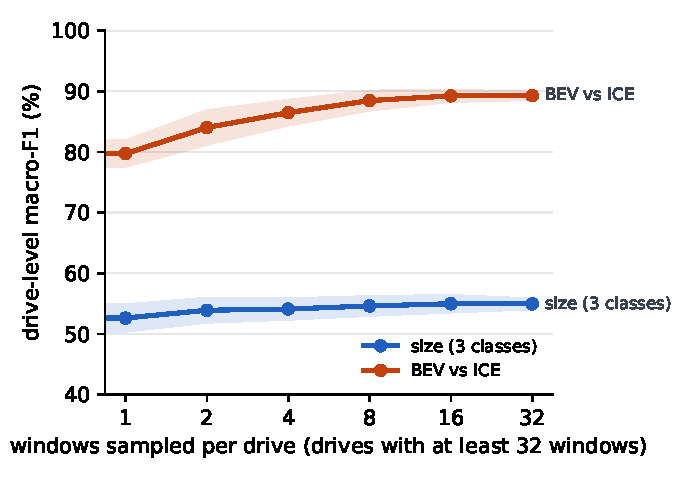
\includegraphics[width=0.85\columnwidth]{evidence_sufficiency.pdf}
\caption{Evidence sufficiency on held-out car models (reference predictions, drive-level macro-F1 in percent): on test drives with at least 32 eligible windows, $m$ windows are drawn per drive and their probability vectors averaged (mean over 50 draws; band: one std). Size moves from 52.6 ($m = 1$) to 54.9 ($m = 32$; all windows 56.0), BEV vs ICE from 79.7 to 89.3 (all windows 89.1), saturating by 8--16 windows.}
\label{fig:evidence}
\end{figure}

\subsection{Ceilings, Separability and Evidence Sufficiency}

Three zero-training oracles bound the size task on the held-out models: a per-car-model majority oracle (every drive of a held-out model gets that model's majority prediction) lifts the ensemble of the 12 reference deep runs from 63.2 to 72.0, so perfect within-model consistency would still leave size far from 90 (BEV vs ICE: 89.8 to 93.5). The footprint-noise oracle of Fig.~\ref{fig:ceiling} scores 92.1 at $\sigma = 0.10$ m$^2$ and 86.6 at 0.15, so reaching 90 needs a footprint error of about $\pm$0.12 m$^2$, about 2.5\% of a 4.6 m$^2$ footprint. A curb-mass oracle (two mass cuts fitted on the training drives) scores 63.3 on the 1,139 test drives with a known mass, so mass is no better proxy.

\begin{figure}[t]
\centering
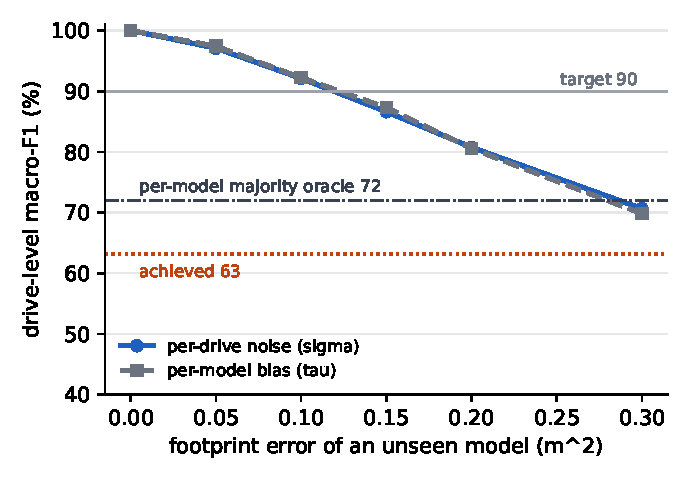
\includegraphics[width=0.85\columnwidth]{footprint_noise_oracle.pdf}
\caption{Footprint-noise oracle for the size task on held-out car models (drive-level macro-F1 in percent, 200 repeats): each drive is classified from the true footprint of its car model plus an error, cut at the fixed thresholds 4.43 and 4.88 m$^2$; per-drive noise of std $\sigma$ (circles) or a per-car-model bias $\tau$ (squares), both in m$^2$. Lines: the reference ensemble of the twelve reference sequence-model runs (63.2), its per-car-model majority oracle (72.0) and the 90 target.}
\label{fig:ceiling}
\end{figure}

The errors sit where the labels are closest: 21 of the 41 held-out car models lie within 0.15 m$^2$ of a differently labelled training model, and in one reference GRU run window accuracy is 53.0\% within 0.1 m$^2$ of a threshold against 89.9\% beyond 0.8 m$^2$. With the reference predictions, LARGE unibody vehicles are read as MID or SMALL while pickups and body-on-frame SUVs are recognised (per-model shares in Section~\ref{sec:discussion}), and MID models just above the 4.43 m$^2$ cut are read as SMALL (drives correct: GWM Haval H6, Audi Q5, Lexus RX and Nissan Altima 0\%, Kia Stinger 25\%).

Evidence per drive is not the limit for the reference models (Fig.~\ref{fig:evidence}): drive accuracy stays between 63.8 and 73.8\% (size) and 85.7 and 93.2\% (BEV vs ICE) from 1--2 to more than 64 windows per drive, and it does not grow with the number of acceleration, deceleration or lead-acceleration episodes.

\subsection{LLM-Proposed Physical Features}

Table~\ref{tab:llm} compares gradient boosting on hand-crafted window statistics, on the 34 registered LLM-proposed features and on both: alone, the physical features are weak per window but strong per drive, on a par with the reference sequence models on BEV vs ICE, and adding the statistics helps size but lowers BEV vs ICE at drive level. By permutation importance of the LLM-features-only gradient boosting on the validation split, BEV vs ICE rests on lift-off deceleration (while moving and shortly after pedal release), the share of deceleration under a pressed accelerator or without the brake, the lead-to-ego deceleration delay and the 10th percentile of brake-free deceleration; size on the curvature-per-steering-angle gain at 6--18 m/s and at low speed, the Ackermann gain at 6--12 m/s and the same delay.

\begin{table}[t]
\centering
\footnotesize
\setlength{\tabcolsep}{3.5pt}
\caption{Gradient boosting on window statistics, on the 34 registered LLM-proposed features and on both (held-out car models, one seed); macro-F1 in percent per window (full and human-only) and per drive (protocol full).}
\label{tab:llm}
\begin{tabular}{@{}lcccccc@{}}
\toprule
 & \multicolumn{3}{c}{Size} & \multicolumn{3}{c}{BEV vs ICE} \\
\cmidrule(lr){2-4} \cmidrule(lr){5-7}
Features & full & human & drive & full & human & drive \\
\midrule
Statistics & 49.7 & 46.3 & 54.7 & 69.5 & 73.5 & 73.2 \\
LLM physical & 40.5 & 47.3 & 63.2 & 69.6 & 84.2 & 89.4 \\
LLM + statistics & 54.1 & 49.8 & 64.9 & 73.2 & 80.2 & 80.9 \\
\bottomrule
\end{tabular}
\end{table}

\subsection{Aggregation and Ensembles}

Out of fold on the reference recipe (GRU and ResNet pooled), the best aggregation variant moves size from 67.5 to 67.8 (+0.3) and down-weighting DAS windows in the mean moves BEV vs ICE from 93.0 to 94.8 (+1.8), short of the pre-registered +1.0 on both tasks, so the plain mean remains the headline. Ensembles stayed below the G4 gate: a GRU + ResNet mean gains under one point over the best member out of fold (BEV vs ICE 93.9 against 93.1--93.5; size 68.8 against 68.2) and stacking is worse (92.3 and 66.5). The supplementary rule fixed before the final test run, the DAS- and episode-weighted log-odds mean of Section~\ref{sec:methods}, moves size from 66.9 to 68.7 on the six final S9 runs (+1.7, 6 of 6 runs improved) and BEV vs ICE from 92.8 to 93.5 on the six B5 runs (+0.7, 6 of 6).

\section{Discussion and Limitations}\label{sec:discussion}

\subsection{Label Resolution, Not Sensing}
Under the fixed footprint cut, 90 drive-level macro-F1 needs each held-out model's footprint to within about $\pm$0.12~m$^2$ (Fig.~\ref{fig:ceiling}). Two curb-mass cuts fitted on training models score only 63.3, and 21 of the 41 held-out car models lie within 0.15~m$^2$ of a differently labelled training model. The gap is set by label resolution and fleet composition, not by model capacity or evidence per drive: architectures stay within about 2 points (Table~\ref{tab:main}) and more windows per drive add little for size (Fig.~\ref{fig:evidence}). Per-model errors (Section~\ref{sec:experiments}) split LARGE by body type: pickups and body-on-frame SUVs are recognised (GMC Yukon, Ford Ranger and Ford F-150 Lightning: 95.5--100\% of drives), while unibody three-row SUVs and full-size sedans are read as MID or SMALL (Genesis G80 and G90, Volkswagen Atlas, Tesla Model~S and Kia EV9: 0--5.6\%), so the networks appear to learn LARGE as a truck's mass-and-driveline signature rather than as footprint.

\subsection{What 90 Needs}
Pooling a vehicle's drives does not rescue size (60.0--62.6 against 66.8--67.1 at drive level): about 45\% of the test vehicles have a single drive and the errors are per car model, so even the per-car-model majority oracle lifts the reference ensemble only from 63.2 to 72.0. Three routes remain: seen car models, as under held-out devices, where the same recipes reach 79.5--80.6 (Table~\ref{tab:device}); the vehicle level for BEV vs ICE, where the GRU B5 rises from 92.6 to 93.4 (95.5 on vehicles with at least two drives) and the ResNet B5 stays at 92.8--93.0; and labels whose margins exceed the resolution of about 0.12~m$^2$, such as cuts in wide gaps of the footprint distribution.

\subsection{Two Protocol Lessons}
First, while a driving automation system (DAS) is engaged, a controller tuned per car model supplies part of the control action. Windows with automation activity are easier for size than windows without (56.4 against 50.2, one bi-GRU run) and harder for BEV vs ICE (79.8 against 84.0, one ResNet B5 run): plausibly the controller carries platform information and masks the pedal behaviour that separates the powertrains. Hence the headline drive-level results (Table~\ref{tab:main}) are paired with the human-only protocol, and the final BEV vs ICE recipe (B5) down-weights DAS windows (the size variant S7 did not win in the fold-0 sweep, Table~\ref{tab:folds}). Second, early stopping on the released validation split, which shares car models with training, selects epochs 16--22, against 1--8 (median about 4) for the reference recipe on the model-disjoint folds (Section~\ref{sec:methods}), and the final models' validation scores do not predict their test scores (Section~\ref{sec:experiments}). Such a split rewards memorising car models, a shortcut~\cite{geirhos2020shortcut}; we therefore fixed the training length from the folds (Table~\ref{tab:folds}), and a future release would carve the validation split model-disjoint.

\subsection{Privacy and Limitations}
Section~\ref{sec:dataset} lists the privacy measures. Labels describe car models, not people: a rare model may be recognisable as a model, never as a person. The same property that makes the data useful, that motion reveals the vehicle, restricts access to research on vehicle dynamics and driving behaviour and prohibits re-identification and linkage with other datasets. Several limitations remain.
All logs come from one logger ecosystem and its software eras~\cite{schafer2018comma2k19}, and the fleet is skewed by region and brand (83.8\% of the hours from North America, 4.8\% from Europe, 4.2\% from Asia); region, software era and device type are metadata, not inputs, but they correlate with powertrain.
Labels are platform attributes: a misidentified platform mislabels every drive of that vehicle, and platforms sold with several powertrains the logs cannot separate, or of unknown powertrain, carry no powertrain label (11.1\% of the drives). On 56.2\% of the drives the lead vehicle comes from a camera model rather than a radar, and pedal magnitudes are missing on 63.9\% (accelerator) and 49.4\% (brake) of the drives. The internal folds never hold out the LARGE~$\times$~BEV cell, which one car model dominates, so their numbers for that cell reflect training models only; the test split does hold out models of that cell.
% Source of the fold statement: CAMPAIGN.md (G1/G2 consequence note) and INTERNAL_FOLDS.md (the LARGE x BEV pool is dominated by one car model); not in OUTLINE.md; verified 8 Nov 2026.
With 41 (size) and 39 (BEV vs ICE) test car models, the GRU recipes' cluster-bootstrap intervals are wide (67.1 [54.4, 74.2] and 92.6 [87.1, 96.2]); differences of a few points between methods lie inside them.

\section{Conclusion}\label{sec:conclusion}
We asked whether a vehicle's size class and powertrain can be read from 60-s windows of trajectory and CAN signals for car models never seen in training. The released dataset (9,062 drives, about 3,950 h, 1,431 pseudonymous vehicles, 174 car models) fixes the labels, the model-disjoint and device-disjoint splits, the window-, drive- and vehicle-level protocols and the cluster-bootstrap intervals over car models. Powertrain is readable: BEV vs ICE reaches 92.6--93.0 drive-level macro-F1 on held-out car models. Size under a footprint cut is only partly readable: a pre-registered campaign raised the bi-GRU drive-level score from 62.9 to 67.1 (point estimates whose bootstrap intervals overlap), four sequence architectures stay within about 2 points, and zero-training oracles show that 90 would need a footprint resolution of about $\pm$0.12~m$^2$, while half of the held-out car models lie within 0.15~m$^2$ of a differently labelled training model. These results are reference points, not a leaderboard. The next steps are labels with margins above that resolution, more fleets and car models, and vehicle-level evaluation where vehicles have several drives.


\ifanonymous\else
\section*{Acknowledgments}
% TODO (authors): funding and acknowledgments, or remove.
\fi

\bibliographystyle{IEEEtran}
\bibliography{refs}

\end{document}
